\documentclass[a4paper,12pt,one side,titlepage]{report}

%en francais
\usepackage[T1]{fontenc}
\usepackage[utf8]{inputenc}
\usepackage[francais]{babel}
%fonts
\usepackage{lmodern}
\usepackage[scaled]{helvet}
\usepackage{fourier}
\usepackage{inconsolata}


\usepackage{amsfonts}
\usepackage{amsmath}
\usepackage{amssymb}
\usepackage{eurosym}
\usepackage{float}
%\usepackage[bottom=2.5cm,left=2.5cm,right=2.5cm]{geometry}
\usepackage[bottom=2.8cm]{geometry}
\usepackage{graphicx}
\usepackage{xcolor}
\usepackage[acronym]{glossaries}
\usepackage[hidelinks]{hyperref}
\usepackage{lipsum}
\usepackage{lastpage}
\usepackage{listings}
\usepackage{pdfpages}
%\usepackage{titlesec}
\usepackage{url}
\usepackage{wrapfig}

\graphicspath{ {../images/} } % dossier img

%lstdefines etc....
\input{codeconf.tex}

\renewcommand{\familydefault}{phv}
%\renewcommand{\familydefault}{\ttdefault}

\newcommand{\selv}{%
\fontfamily{phv}\fontseries{b}\fontsize{8}{20}\selectfont}
\newcommand{\belv}{%
\fontfamily{phv}\fontseries{b}\fontsize{10}{22}\selectfont}
\newcommand{\telv}{%
\fontfamily{phv}\fontseries{l}\fontsize{12}{22}\selectfont}
\newcommand{\inco}{%
\fontfamily{\ttdefault}\fontseries{b}\fontsize{10}{10}\selectfont}
\newcommand{\ipath}[1]{{\inco \normalsize {#1}}}
%\newcommand{\fnu}[1]{\footnote{\url{#1}}}
\newcommand{\fnu}[2][]{\footnote{{#1}\url{#2}}}


%%% header & footer
% \leftmark : afficher nom section
\usepackage{fancyhdr}
\pagestyle{fancy}
\renewcommand{\headrulewidth}{1pt}
\fancyhead[C]{\selv\leftmark}
\fancyhead[L]{\selv ELK}
\fancyhead[R]{\selv Équipe réseau Lothaire}%\includegraphics[width=60px]{openstack-logo.png}}

\renewcommand{\footrulewidth}{0pt}
\fancyfoot[C]{\telv Page \thepage\hspace{2px} / \pageref{LastPage}} 
\fancyfoot[L]{\includegraphics[height=20px]{elasticmini.png}}
\fancyfoot[R]{\belv François \textsc{Dupont}}



%Titre et Auteurs
%\title{Architecture pour l'hébergement web à fort trafic}
%\author{Auteurs : \textit{Dupont Francois}\\\\Tuteur : \textit{Vincent Delove}}
%\date{Lundi 23 Mars 2015}


\newglossaryentry{API}{name={API},
                             description={Une API, Application Programming Interface, est une interface permettant d'interagir avec un programme par l'intermédiaire d'"opérations simples". Elles sont en générale la pour faciliter la réutilisation d'un programme plus complexe. C'est parce que openstreetmap à une API que l'on a vu autant de logiciels utilisant ses cartes/tuiles.
}}

\newglossaryentry{cron}{name={cron},
                             description={Cron est un gestionnaire de tâche automatique sur linux, il est extremement répendu.
}}
\newglossaryentry{flag}{name={flag},
                             description={Un drapeau, dans la dénomination logstash, le flag représente une option passé en argument exemple : -w.
}}

\newglossaryentry{cluster}{name={cluster},
                             description={Cluster ou grappe. Un cluster est constitué d'un ou plusieurs nodes qui partagent le même \emph{cluster.name}
}}

\newglossaryentry{document}{name={document},
                             description={Un document, dans la terminologie elasticsearch, est constitué d'un ou plusieurs nodes qui partagent le même \emph{cluster.name}
}}

\newglossaryentry{fulltext}{name={fulltext},
                             description={Un drapeau, dans la dénomination logstash, le flag représente une option passé en argument exemple : -w.
}}

\newglossaryentry{index}{name={index},
                             description={Un index dans la terminologie est ce qui se rapproche d'une base dans le modèle relationnel \emph{classique}. 
}}

\newglossaryentry{lucene}{name={lucene},
                             description={Apache Lucene 
}}
\newglossaryentry{logs}{name={logs},
                             description={Un log c'est une buche !
}}

\newglossaryentry{mapping}{name={mapping},
                             description={Le mapping. Dans la terminologie elasticsearch, un node est processus java 
}}

\newglossaryentry{node}{name={node},
                             description={Node ou noeud est, dans la terminologie elasticsearch, un processus  processus java lucene, c'est une instance d'elasticsearch. 
}}

\newglossaryentry{shard}{name={shard},
                             description={Dans la terminologie elasticsearch, un shard est un index ou un morceau d'index. C'est un index au sens lucene du terme. Il existe deux types de shards, des shards primaires et des shards répliqués. Un shard primaire peut indexer de nouvelles données alors qu'un shard repliqué sert seulement de failover, il peut également être utilisé pour accélérer les réponses aux requêtes.
}}


\newglossaryentry{thread}{name={thread},
                             description={explication thread processus etc.. 
}}

\newglossaryentry{type}{name={type},
                             description={Un type dans la terminologie elasticsearch est l'équivalent d'une table dans le modèle relationnel. Il est équivalent dans la mesure où il possède des champs contenant des valeurs
}}

%\newglossaryentry{BGP}{name={BGP},
%                             description={BGP, Border Gateway Protocle, est un protocole d'échange de routes utilisé sur internet, il permet aux AS (autonomous systems) d'échanger leurs informations.\\
%                             Le plus connu des mauvais usages de BGP s'est produit en février 2008 lorsque Pakistan Telecom a mal appliqué une demande de censure de YouTube, le rendant indisponible pour le monde entier pendant plusieurs heures.\\
%                             Le black-holing BGP est une technique d'endiguement de DDOS souvent utilisée en dernier recours. Pour protéger l'infrastructure réseau (d'un FAI par exemple), on décide que tous les accès à une IP/un range d'IP seront redirigés vers NULL. }}
%\newglossaryentry{CLI}
%{
%	name={CLI},
%	description={Command Line Interface: interface en ligne de commande, se dit d'un programme auquel on accède par l'intermédiaire d'un shell (terminal en ligne de commande). Ces programmes sont en général légers puisqu'ils sont entièrement textuels.}
%}
%
%\newglossaryentry{DDOS}{name={DDOS},
%                        description={Distributed Denial Of Service ou attaque par déni de service distribué. Attaque informatique ayant pour objectif de rendre indisponible un service, un site web etc... en saturant le serveur qui l'héberge (il existe de nombreux type de DDOS différents)}}
%
%\newglossaryentry{firewall}{name={firewall},
%                             description={Pare-feu : système de protection réseau pour un ordinateur ou un réseau d'ordinateur, dans ce projet nous parlerons essentiellement de pare-feu logiciel}}
%
%\newglossaryentry{failover}
%{
%	name={failover},
%	description={Un failover, traduit par passer outre à la panne, est la capacité d'un équipement à basculer automatiquement vers un réseau alternatif ou en veille.}
%}
%
%\newglossaryentry{jumbo frames}{ name={jumbo frames},
%                                description={En réseau, des jumbos frames sont des trames Ethernet dont la longueur dépasse 1500 octets. En général, les jumbo frames peuvent avoir une longueur allant jusqu'à 9000 environ octets.}
%}
%
%\newglossaryentry{hash}
%{
%	name={hash},
%	description={On nomme fonction de hachage une fonction particulière qui, à partir d'une donnée fournie en entrée, calcule une empreinte servant à identifier rapidement, bien qu'incomplètement, la donnée initiale. Les fonctions de hachage sont utilisées en informatique et en cryptographie.}
%}
%
%\newglossaryentry{load balancer}{ name={load balancer},
%                                description={Un répartisseur de charge, ou load balancer, est un ensemble de techniques permettant de distribuer la charge de travail entre plusieurs ordinateurs d'un groupe}
%}
%
%\newglossaryentry{naxsi}
%{
%	name={naxsi},
%	description={Un type de firewall}
%}
%
%\newglossaryentry{OSI}{ name={OSI},
%                                description={Open System Interconnection model est un modèle conceptuel qui caractérise et standardise les communications sur internet. Ce modèle a été standardisé dans l'ISO/IEC 7498-1 (International Organization for Standardization). Il possède 7 couches. 
%                                Réparties comme suit :\\
%    \begin{tabular}{|c|c|c|}
%        \hline
%        Numéro& Couche       & Exemple de protocole\\
%        \hline
%        7&      Applications &  HTTP, NFS, DHCP, BGP, DNS etc... \\
%        \hline
%        6&      Présentation &  MIME, SSL\\ 
%        \hline
%        5&      Session      &  Sockets, SOCKS, NetBIOS\\
%        \hline
%        4&      Transport    & TCP, UDP\\
%        \hline
%        3&      Réseau       & IP4/6, IPsec\\
%        \hline
%        2&      Liaison      & PPP, Token Ring, CRC,\\
%        \hline
%        1&      Physique     & Wifi, Ethernet, CAN, RS-232\\
%        \hline
%    \end{tabular}
%                                }
%}
%
%\newglossaryentry{overhead}
%{
%	name={overhead},
%	description={Coût supplémentaire engendré pour atteindre un but (cette définition est agnostique à la méthode ou la technologie).\\
%    Exemple : Envoyer "Bonjour" à un correspondant par internet (disons sur un chat en ligne), ici la charge utile est "Bonjour"\\
%    Une fois le message enregistré il va être encapsulé de nombreuses fois (TCP, HTTP, conversion en binaire pour la couche physique, etc..)
%    pour être affiché chez notre correspondant. Tout cela prend du temps de calcul, du temps de transport, de la "place" (envoyer toutes
%    ces en-têtes multiplie plusieurs fois la taille du message original). La différence entre le payload (la charge utile originale) et le
%    résultat final est appelé overhead.
%    }
%}
%
%\newglossaryentry{scalabiliser}{ name={scalabiliser},
%                                description={Scalabiliser est un anglicisme courant signifiant mettre à l'échelle. On parle de mise à l'échelle lorsqu'une infrastructure a la capacité de démultiplier sa capacité de traitement. On attend en général que cette mise à l'échelle soit rapide, voire automatisée.}
%}
%
%\newglossaryentry{SSL}
%{
%	name={SSL},
%	description={Secure Socket Layer est un protocole de sécurité SSL qui fonctionne suivant un mode client-serveur. Il permet de satisfaire aux objectifs de sécurité suivants :\begin{itemize}
%	\item l'authentification du serveur.
%	\item la confidentialité des données échangées (ou session chiffrée).
%	\item l'intégrité des données échangées.
%	\end{itemize}
%    voir aussi \gls{TLS}}
%}
%
%\newglossaryentry{TLS}
%{
%	name={TLS},
%	description={Transport Layer Security est une évolution du protocole SSL : cf \gls{SSL}}
%}
%
%\newglossaryentry{wireshark}
%{
%	name={wireshark},
%	description={Wireshark est un analyseur de paquets libre utilisé dans le dépannage et l'analyse de réseaux informatiques, le développement de protocoles, l'éducation et la rétro-ingénierie. Wireshark permet d'analyser les paquets qui transitent sur un réseau en les interceptant.}
%}
%
%
%
%
%
%
%parser


\makeglossaries

\begin{document}

\begin{titlepage}
\begin{center}
 \newcommand{\HRule}{\rule{\linewidth}{0.5mm}}

%\includegraphics[width=0.15\textwidth]{debian.png}~\\[1cm]
\includegraphics[width=0.6\textwidth]{Logo-IUT-UL.jpg}\\[1cm]

%\textsc{\LARGE University of Beer}\\[1.5cm]

\textsc{\LARGE Licence ASRALL}\\[0.5cm]

% Title
\HRule \\[0.4cm]
{ \Large \bfseries Déploiement d'ELK pour l'analyse de log\\[0.4cm] }

\HRule \\[1.5cm]

% Author and supervisor
\noindent
\begin{minipage}{0.5\textwidth}
\begin{flushleft} \large
\emph{Auteur:}\\
François \textsc{Dupont}\\
\end{flushleft}
\end{minipage}%
\begin{minipage}{0.5\textwidth}
\begin{flushright} \large
\emph{Tuteur:} \\
Vincent \textsc{Delove}
\end{flushright}
\end{minipage}

%

\vfill

\begin{figure}[h]
    \centering
    \includegraphics[scale=0.5]{logstash.png}
    %\hspace{10mm}
    \hfill
    \includegraphics[scale=1]{kibana.png}
    \\[0.2cm]
    \includegraphics[scale=1]{lothaire.jpg}
    \hfill
    \includegraphics[scale=0.6]{elasticsearch.png}
    \\
    \includegraphics[scale=0.4]{elastic.png}
\end{figure}

% Bottom of the page
\vfill
{\today}%Lundi 23 Mars 2015}

\end{center}
\end{titlepage}




%Page remerciments
\emph{\Large Remerciements}
\\[2cm]
Je tiens tout d'abord à remercier Vincent \textsc{Delove} mon maître de stage pour 
m'avoir proposé le sujet, mais également pour son support, ses conseils, sa patience
et sa disponibilité.
\\[2cm]
Je remercie également Emanuel \textsc{Nataf} mon tuteur pour  son intérêt pour mon 
sujet ainsi que les marges de manoeuvres qu'il à su me laisser.
\\[1cm]
Merci à toute l'équipe du réseau Lothaire pour son accueil chaleureux et son soutien.
Je remercie plus particulièrement  Luc \textsc{Didry} et Stéphane \textsc{Fetter} pour leur
aide, en général, et  notamment en système.

%Page table des matières
\setcounter{tocdepth}{1}
\tableofcontents

%%%%%%%%%%%%%%%%%%%%%%%%%%%%%%%%%%%%%%%%%%%%%%%%%%%%%%%%%%%%%%%%%
%Introduction
\part{Introduction}

\chapter{Introduction}
\section{Problématique}
La gestion de \gls{logs} est une problématique commune à presque tous les services informatiques,
tous les fournisseurs de services et plus globalement, toutes personnes gérant une infrastructure 
informatisée.

Les \gls{logs} sont précieux car ils sont un des éléments indispensables au dépannage, 
au monitoring. Ils permettent d'anticiper des problèmes inhérents à l'exploitation 
des infrastructures, et  de constater de potentielles tentatives d'intrusions.
À ces aspects pratiques relatifs au bon fonctionnement des systèmes s'ajoute également
une problématique judiciaire. Il est souvent nécessaire de garder des logs pour un 
temps défini  dans la loi. Ces logs doivent évidemment être consultables de manière
diligente.

Avec des milliers de lignes de logs par seconde, il est devenu impossible de naviguer
"au hasard" dans les fichiers pour regarder si tout se passe bien.

Cependant, \emph{de nombreuses structures continuent encore aujourd'hui d'analyser 
plus ou moins "manuellement" leurs \emph{\gls{logs}}}. Cette méthode reste envisageable 
si on cherche quelque chose de précis, comme une IP dans un intervalle de quelques 
secondes, mais impossible pour des recherches trop vagues, on se noie.


\section{Objectif}
En résumé, l'objectif de ce projet est de redonner la possibilité aux administrateurs
de vérifier le bon fonctionnement de leur infrastructure sans avoir à attendre l'alerte
Nagios (qui reste indispensable). L'idée est de permettre un suivi quotidien, permettant
de mettre en évidence des indicateurs de bonne ou de mauvaise santé du système, sans 
pour autant que ces problèmes soient critiques (mieux le système est entretenu, moins
on risque la panne).
Pour réaliser ce projet il a été décidé d'utiliser la stack ELK\footnote{Elasticsearch Logstash Kibana}.



\subsection{Limites}
Pour des raisons de disponibilité matériel mais, aussi, d'intérêt par rapport au sujet,
je n'ai pas travaillé sur les clusters Elasticsearch de façon pratique. Elasticsearch
est un logiciel hautement parallélisable, et qui donc scale très bien à l'horizontal. 

Ce rapport se concentre sur l'aspect gestion de logs, il est possible de faire bien
plus avec Elasticsearch que ce qui est présenté dans ce rapport.
De même nous nous concentrons avec logstash sur l'exploitation de syslogs. Il est 
capable de faire d'autres choses, notamment, avec les logs apache. On présentera 
tout de même une base solide de ce qui est faisable avec.


\section{Organisation du rapport}
La première partie du rapport sera consacrée à l'environnement de travail et à la 
présentation des notions. La seconde se concentrera sur le fonctionnement de chacun 
des logiciels utilisés ainsi que quelques problèmes liés à leur exploitation en production.
Enfin la troisième partie conclura ce rapport en présentant la solution retenue 
pour la mise en production, les éventuels ajouts possibles.

\chapter{Environnement}
J'ai réalisé mon stage de Licence professionnelle ASRALL, dans l'équipe réseau Lothaire.
Cette équipe dépend de la Sous Direction des Infrastructures, membre de la Direction 
du numérique de l'Université de Lorraine. Son rôle est d'opérer le réseau des 
établissements scolaires et de recherche de la région Lorraine.
\section{Réseau Lothaire}
\begin{figure}[H]
\center
\includegraphics{lothaire.jpg}
\end{figure}
Le réseau de télécommunications à haut débit sur le territoire de la région Lorraine, 
dénommé Lothaire, est réservé aux secteurs de l’Enseignement Supérieur, de la Recherche 
et du Transfert de Technologie. 

L'équipe Lothaire assure l’interconnexion des réseaux de Nancy (\emph{StanNet}), 
Metz (\emph{AmpereNet}), Epinal (\emph{EpiNet}) ainsi que d'autres sites en région 
(IUFM, CROUS\ldots) avec le réseau \emph{RENATER} (REseau NAtional de télécommunication 
pour la Technologie, l'Enseignement et la Recherche). Ce lien est réalisé au nœud 
régional situé sur le site du Montet (mon lieu de stage) à Vandœuvre-lès-Nancy.

(cf \hyperref[fig:imagereseaulothaire1]{schéma 10.1}  et \hyperref[fig:imagereseaulothaire1]{schéma 10.2} 
en annexes)

\subsection{Historique et rôle et organigrame}

Avant la création de \emph{l'Université de Lorraine} au 1er Janvier 2012 l'équipe 
réseau Lothaire était attachée au CIRIL (Centre Interuniversitaire de Ressources Informatiques
de Lorraine). Depuis, l'organisme a été absorbé par la sous direction des infrastructure
de l'université.

En plus d’opérer les infrastructures du réseau Régional, l’ Equipe Réseau Lothaire 
assure un ensemble de services auprès de la Communauté de l’Enseignement Supérieur 
et de la Recherche de Lorraine :

\begin{itemize}
    \item interface technique et financière avec les établissements partenaires, 
    les opérateurs et les prestataires retenus,
    \item configuration du routage (IPv4 et IPv6) et des règles de sécurité (ACL , 
    Firewall),
    \item service de gestion des noms de domaines (DNS),
    \item développement, maintenance et diffusion nationale d’outils de métrologie ,
    \item administration d’un portail captif (YaCaP) pour les accès Wifi,
    \item filtrage des accès WEB sur certains réseaux,
    \item gestion d’une plateforme pour les accès sécurisés (VPN),
    \item collecte et archivage des traces (logs) des activités réseaux,
    \item mise à disposition de logiciels libres pour la communauté (FTP),
    \item service de synchronisation d’horloge (NTP),
    \item routage d’appel de visioconférences (gatekeeper H323),
    \item gestion des réseaux de campus de l’Université de Lorraine.
\end{itemize}                                                

L'équipe est constituée de 10 ingénieurs, dont 1 responsable Alexandre Simon, ainsi
que d'un enseignant chercheur détaché.


\section{Environnement de travail}
J'ai physiquement réalisé mon stage dans un bureau (plutôt spacieux), en compagnie
d'un autre stagiaire.
Ma machine travail était un ordinateur fixe Dell Optiplex 780 équipé d'un Core2 et 
de 4 Go de RAM. Il m'a été laissé une grande liberté quant à l'installation de mon
système d'exploitation, j'ai donc choisi un classique Debain GNU/Linux.

Cette machine était bien pratique pour réaliser des tests (machines virtuelles, 
installation de logiciels\ldots), mais n'était évidemment pas capable d'ingurgiter 
tous les logs réseau des établissements d'enseignement en Lorraine. On a donc mis 
à ma disposition (dans le Datacenter du bâtiment) 2 serveurs qui serviront après 
la fin du stage de machines de production. Un Dell R520 (12 cœurs, 12Go de RAM),
c'est la machine qui fera tourné Elasticsearch et un Dell 2950 (4 coeurs 4 Go de RAM)
c'est la machine qui accueillera le Logstash qui traitera tous les logs.

Par cohérence avec le reste de l'infrastructure il a été décidé d'installer une 
Debian Jessie, nouvellement stable au moment de l'installation.
%\chapter{La gestion de logs}
%
%La gestion des \gls{logs} est un problème presque aussi vieux que l'informatique.
%Au commencement 
%
%La tendance est cependant (et depuis longtemps) à la centralisation de ces fichiers afin de faciliter 
%leur accès et leur analyse ultérieur. Cela permet également une sauvegarde plus facile de ces derniers 
%dans le cas où cela est nécessaire. Il est fréquent d'avoir des scripts analysant 
%quotidiennement ces \gls{logs} afin de pouvoir détécter un comportement suspect.
%
%
%\chapter{Gestion de projet}
%%\section{Tableau de bord}

\begin{table}[h]
\begin{tabular}{lllllll}
\hline
\multicolumn{7}{c}{Tableau de bord}                                  \\\hline
Semaine &\vline\hspace{1mm} Lundi &\vline\hspace{1mm} Mardi &\vline\hspace{1mm}
Mercredi &\vline\hspace{1mm} Jeudi &\vline\hspace{1mm} Vendredi &\vline\hspace{1mm} Commentaires \\\hline
1       &       &       &          &       &          &              \\\hline
2       &       &       &          &       &          &              \\\hline
3       &       &       &          &       &          &              \\\hline
4       &       &       &          &       &          &              \\\hline
5       &       &       &          &       &          &              \\\hline
6       &       &       &          &       &          &              \\\hline
7       &       &       &          &       &          &              \\\hline
8       &       &       &          &       &          &              \\\hline
9       &       &       &          &       &          &              \\\hline
10      &       &       &          &       &          &              \\\hline
11      &       &       &          &       &          &              \\\hline
12      &       &       &          &       &          &             
\end{tabular}
\caption{Tableau de bord}
\centering
\end{table}

%\chapter{Présentation des notions}
%\chapter{Définitions}

\part{Les logiciels}
\chapter{Logstash}
\begin{figure}[H]
\center
\includegraphics[width=0.2\textwidth]{logstash.png}
\label{fig:logstashlogo.png}
\end{figure}
\section{Présentation de Logstash}

\subsection{Pourquoi Logstash?}
Bien qu'un administrateur système compétent soit capable d'analyser de façon rapide 
et efficace les logs d'une machine (à l'aide deperl+awk+sed+tail+grep), cette méthode
est fastidieuse. De plus, face à des dizaines/milliers de machines (virtuelles aussi), 
cette méthode n'est plus applicable, elle ne peut pas passer à l'échelle.
Il est actuellement fréquent (cloud, applications multicouche, \ldots) que les logs 
d'une seule machine ne suffise plus à diagnostiquer le problème auquel on est confronté.

\subsection{Fonctionnement interne}
L'utilisation de logstash est un pipeline qui s'articule autour de 3 \emph{blocs} 
également appelés \emph{stages} (phase).
\begin{itemize}
    \item   Le bloc : \emph{Inputs} génère des événements à partir des informations reçues
    par logstash en entrée.
    \item   Le bloc : \emph{Filters} modifie, manipule, ces évènements dans logstash
    \item   Le bloc : \emph{Outputs} envoie les évènements de logstash vers leur 
    prochaine destination.
\end{itemize}

Cette façon de fonctionner peut faire penser à \emph{iptables}.

Logstash est un logiciel développé en Jruby\footnote{sauf mention contraire, on supposera
dans ce rapport que logstash est développé en ruby} (Jruby est en faite une implémentation
de ruby 1.8 en Java qui était à l'époque plus rapide que ruby "seul"). 
Le passage d'une phase à l'autre est implémenté via les \emph{SizedQueue} de ruby. 
Elles sont dimensionnées pour contenir 20 éléments\footnote{appelés messages lorsqu'on parle de queues, on parle bien ici 
des \textbf{événements} logstash}, ce n'est pas paramétrable sans modifier le code 
source, c'est un choix délibéré. Ces queues ne sont pas conçues pour stocker des 
données à long terme. On verra plus tard que ce la justifie l'utilisation d'un 
\textit{buffer}, comme \emph{Redis}\footnote{voir la sous partie sur la tolérence
de pannes ainsi que le chapitre consacré à Redis}.


Chaque bloc est composé d'une multitude de plugins. Ce sont des modules indépendants
qui peuvent également fonctionner en conjonction les uns des autres.

Il est, par exemple, possible de configure le bloc \emph{inputs} pour utiliser 
plusieurs fois le plugin "file" (on imagine pour des cas d'utilisation différents) 
et de se servir dans le même temps d'un autre plugin du bloc \emph{inputs} : stdin 
qui prendra typiquement en entrée le clavier.


Il est possible d'implémenter de nouveaux plugins en ruby afin de les ajouter à
notre logstash.

Il existe également un \textit{pseudo-bloc} qui peut s'insérer dans les autres, ce 
bloc, \emph{codec} permet la de gérer la \textit{représentation des données} c'est 
à dire qu'un codec est capable de lire ou d'écrire dans une syntaxe particulière 
comme par exemple rubydebug, collectd, ou, bien plus intéressant pour nous, netflow.

%wtf why?
%et les types ??


%Explications supplémentaires sur les filtres
% les plugins et les patterns par défaut?

\subsubsection{Tolérance de pannes}
Vos logs sont \textbf{importants}, c'est la raison d'être de Logstash, il ne souhaite 
pas que vous en perdiez le moindre à cause d'un problème réseau ou d'une défaillance
quelconque rendant la destination indisponible.
%cf pipeline.rb et base.rb dans github
Lors d'une indisponibilité, les plugins outputs tentent de renvoyer les événements 
vers leur destination. Si ce n'est pas possible le plugin arrête de lire sa queue 
tant que le message n'a pas pu être envoyé. Par effet domino, une fois la queue 
\textit{filtre => output} remplie, le bloc filtre, ne pouvant plus envoyer de nouveaux 
messages à la queue \textit{FO}. Le plugin du bloc filtre va également retenter 
d'envoyer ses messages, et refuser en attendant de lire les nouveaux arrivant dans 
la queue \textit{input => filtre}.
Si cette dernière venait à se remplir c'est le Logstash tout entier qui refuserait de 
traiter de nouvelles informations. Dans le meilleur des mondes, les expéditeurs de
données se comporterais comme logstash et attendraient patiemment que le problème
se résolve, malheureusement cela n'est pas toujours possible, particulièrement dans
nos problématiques d'où l'importance d'un Redis en amont (ou en aval) afin de 
faire tampon.\footnote{Il existe d'autres outils que Redis, (dont ce n'est pas la fonction
principale) pour réaliser ce travail, ils sont plus adapté mais aussi moins documentés
dans leur utilisation avec logstash.}

\subsubsection{Multithread}
Attention ces informations sont pour le moment, \date{Jeudi 16 Avril}, correctes 
mais sont amenées à changer, notamment concernant les outputs.

Chaque plugin utilise input un \gls{thread}, cela permet d'éviter les engorgements si  
certaines entrées sont plus longues à traiter que d'autres.

En le bloc filtre entier n'utilise par défaut qu'un seul thread, mais il est possible 
d'augmenter le nombre de threads affectés au traitement des filtres avec le \gls{flag}
-w lors du démarrage de Logstash.

À l'heure actuelle le bloc output de logstash ne peut utiliser qu'un seul thread.
Il lit donc sa queue de façon séquentielle.


\section{Installation}
%Sur debian il n'existe pas de paquet deb déjà fait, et le seul prérequis 
%est d'avoir une version de java > 1.7.0\_45
%Pour télécharger et installer
%curl -O https://download.elasticsearch.org/logstash/logstash/logstash-1.4.2.tar.gz
%
%tar zxvf logstash-1.4.2.tar.gz
%
%script before-install.sh
%
%sudo cp -r /home/\$USER/Downloads/logstash-1.4.2 /opt/logstash
%
%sudo mkdir /var/log/logstash
%
%script after-install.sh
%
%cd logstash-1.4.2
%
%Création du path
%
%export PATH+=:/opt/logstash
%
%Dautres méthodes d'installation

%Ensuite un simple git clone https://github.com/elastic/logstash.git
%nous permet de récupérer le dépot stable le plus récent.
%Enfin des scripts d'installation sont disponible
%dans logstash/pkg/debian



Sur Debian jessie il n'existe pas de paquet officiel logstash maintenu. Il existe 
en revanche un paquet tiers\fnu{https://download.elastic.co/logstash/logstash/packages/debian/logstash\_1.4.2-1-2c0f5a1\_all.deb}
fourni par l'éditeur du logiciel. Le dit paquet n'est pas de très bonne facture  
puisqu'il nécessite l'ajout de dépendances manuelles\footnote{wget paquet, 
dpkg -i paquet, apt-get install -f} ainsi qu'un rechargement de 
la configuration des services : \emph{systemctl daemon-reload}.

Les dépendances nécessaires sont \emph{jruby} et \emph{openjdk-7-jre}, les mêmes 
que pour elasticsearch.

Une autre manière de réaliser l'installation est d'ajouter les dépots logstash à 
\ipath{/etc/apt/source.list.d/logstash.list.d/logstash.list}

\begin{lstlisting}[style=code,label={lst:ajoutdepotlogstash}]
deb https://packages.elasticsearch.org/logstash/1.4/debian stable main
\end{lstlisting}

et évidemment la clef qui va bien\footnote{permet d'authentifier les paquets téléchargés
(cf:SecureApt)}

\begin{lstlisting}[style=code,label={lst:ajoutclefdepotlogstash}]
wget -qO - https://packages.elasticsearch.org/GPG-KEY-elasticsearch | sudo apt-key add -
\end{lstlisting}

\subsection{Configurations}
Il est d'usage dans une installation \textit{propre} de créer un utilisateur spécifique
à notre utilisation. C'est également le cas dans notre paquet. L'administrateur 
système doit donner à cet utilisateur, nouvellement créer les droits nécessaire 
pour qu'il puisse faire son travail correctement correctement. Dans le cadre de 
l'analyse de log faire de l'utilisateur logstash un membre du groupe \emph{adm}, 
le groupe d'administration de Debian lui permettra par exemple d'avoir accès en 
lecture à la plupart des fichiers de \ipath{/var/log/}.

\subsubsection{Set Capabilities}
Cependant cette façon de faire peut ne pas être suffisante.
Notre utilisation de logstash consiste, entre autre, à centraliser les \gls{logs}. 
Ces derniers sont généralement envoyés par l'intermédiaire de syslog (RFC 5244).
Par défaut syslog utilise le port 514, ce port est inférieur à 1024, et donc \textit{privilégié}.
Aussi seul \emph{root} à le droit d'écouter ces ports. Ajouter notre utilisateur 
logstash au groupe root enlèverait le bénéfice de sécurité obtenu en isolant les 
utilisateurs en fonction de leurs besoins. Nous allons plutôt utiliser les 
\emph{capabilities}\fnu{http://man7.org/linux/man-pages/man7/capabilities.7.html} 
et la commande \emph{setcap}\fnu{https://github.com/elastic/logstash/issues/1587}
\begin{lstlisting}[style=code,label={lst:setcapabilities}]
setcap cap_net_bind_service=+epi /usr/lib/jvm/java-7-openjdk-amd64/jre/bin/java
setcap cap_net_bind_service=+epi /usr/lib/jvm/java-1.7.0-openjdk-amd64/jre/bin/java
\end{lstlisting}
qui permettent à un processus (thread en faite) de ne pas se soumettre à certaines 
vérifications de sécurité du noyau.

\textbf{cap\_net\_bind\_service} permet à un utilisateur non privilégié (non root) 
d'écouter sur les ports privilégiés.

Les informations concernants les autres capabilities existants sont disponible dans
la page de manuel correspondante : \emph{man capabilities}.

\textbf{=+epi} signifie que l'on ajoute une \emph{capapbility} à un fichier. Plus 
précisement \textbf{=+} signifie que l'on écrase les droits précédents pour les remplacer
par les nouveaux. \textbf{e, p} et \textbf{i} sont la gradation de droits que l'on peut 
attribuer à un fichier avec les capabilities\fnu{https://www.kernel.org/pub/linux/libs/security/linux-privs/kernel-2.2/capfaq-0.2.txt}. 

\begin{itemize}
    \item \textbf{effective}: indique si la capability est utilisé actuellement
    \item \textbf{permited}: définit quelles capabilities sont autorisé pour un 
    processus donné
    \item \textbf{inherited}: permet de transmettre la capability à un autre programme
\end{itemize}
\textbf{Note}: par défaut, changer le propriétaire d'un fichier de root, à non root enlève
les capabilities associées à ce dernier\footnote{\scriptsize{http://stackoverflow.com/questions/17743062/changing-user-ids-for-assigning-additional-capabilities}}.

Pour vérifier les \textit{capabilities} d'un binaire on utilise la commande 
\emph{getcap}.

\begin{lstlisting}[style=code,label={lst:getcapabilities}]
    getcap /bin/ping
    /bin/ping = cap_net_raw+ep
\end{lstlisting}

Pour les enlever les capabilities il faut utiliser la commande suivante.
\begin{lstlisting}[style=code,label={lst:unsetcapabilities}]
setcap cap_net_bind_service=-epi /usr/lib/jvm/java-1.7.0-openjdk-amd64/jre/bin/java
\end{lstlisting}

Enfin, il est possible, de donner le droit à un utilisateur non root, l'autorisation
de modifier certaines capabilities. Pour ce faire, il faut modifier le fichier \\[1mm]
\ipath{/etc/security/capability.conf}.

%\subsection{Installation de plugins tiers}
%Procédure pour l'installation d'un plugin tiers

\section{Fonctionnement}
\subsection{La base}
Grossièrement Logstash permet traiter et transférer des données, en masse. Nous ne
l'utiliserons essentiellement qu'avec Elasticsearch en utilitaire de sorti. Cependant
et comme le montre la liste des ses abondants plugins d'output, Logstash est capable
de fonctionner avec de nombreux autres logiciels.


\section{Grammaire et conjugaison}
\subsection{Généralités}
Dans cette section nous allons brièvement expliquer le fonctionnement de la syntaxe 
du fichier de configuration de Logstash.\fnu{http ://logstash.net/docs/1.4.2/configuration}

Le ou les fichiers de configuration comportent deux ou trois parties, représentant 
les blocs dont nous avons parlé au préalable. Le bloc \emph{filter} est optionnel
et il est important de noter que, si il est possible de répartir sa configuration
dans plusieurs fichiers, cette dernière sera concaténer, attention aux boucles infinies
dans ce cas là.

\begin{lstlisting}[style=logstash,label={lst:conflogstashminimale},caption={Configuration minimale}]
input {
    stdin{}#ceci est un plugin
}

#filter {
#}#on peut également commenter en fin de ligne

output {
    stdout{}#ceci est un autre plugin
}
\end{lstlisting}

Ici on constate l'utilisation des plugins stdin et stdout, stdin. Comme leur nom 
et leur emplacement dans le fichier de configuration peut le laisser supposer.
Ici Logstash collecte en entrée tout ce qui vient de l'entrée standard, typiquement
le clavier, et l'envoie sur la sortie standard, typiquement, un terminal.
Pour pouvoir recevoir l'output, il est d'ailleurs conseillé d'utiliser, le flag -f
et de ne pas lancer logstash en mode daemon.

Dans ce second exemple, plus complexe, nous allons présenter une utilisation plus
vaste des plugins et la logique sous-jacente à leur utilisation.

\begin{lstlisting}[style=logstash,label={lst:conflogstashiniteloop},caption={Infinite loop}]
#mail.conf
input {
    file {
        path => ["/home/fdupont/testmail"]
    }
}

filter{
    throttle{
        before_count => 2
        after_count => 4
        period => 120
        key => "%{message}"
        add_tag => "contenu"
    }
}

output {
    stdout{ }
    if "contenu" not in [tags]{
        email{
            to => "fdupont@localhost"
            from => "logstash@%{host}"
            subject => "%{message}"
            body => "Ceci est un test sur l'hote %{host}\n avec pour message : %{message}"
        }
    }
}

#shipping.conf
input {
    file {
        path => ["/var/log/secure", "/var/log/messages", "/var/log/*.log","/var/mail/fdupont"]
        exclude => ["*.gz"]
    }
    file {
        path => ["/var/mail/ldidry"]
    }
}


output {
    stdout{ }
    redis {
        host => "100.127.255.1"
        data_type => "list"
        key => "logstash"
    }
}
\end{lstlisting}

Cet exemple de code ne dois pas être utilisé : c'est une boucle infinie.
Il permet en revanche d'expliquer de nombreux points de fonctionnement de la syntaxe
du fichier de configuration de Logstash.
Ce code représente en faite {\bfseries 2 fichiers}, mail.conf et shipping.conf, tout
deux situés dans le répertoire par défaut des fichiers de configuration de Logstash
\ipath{/etc/logstash/conf.d/}. Ils sont lus par ordre alphabétique et concaténés 
(comprendre que les inputs ainsi que les outputs sont fusionnés, il faut donc être
rigoureux dans leur écriture afin de ne pas créer d'effets de bord indésirables).
Une bonne pratique consiste, à utiliser la convention de nommage suivante : \textit{
00-description, 01-description} etc \ldots


Chacun possède un bloc input, output et l'un d'entre eux : filter.
Dans chacun des blocs on trouve un ou plusieurs {\bfseries plugins} comme email, 
file, redis ou d'autres. 
Chacun de ces plugins possède son propre paramétrage, réglable au travers de 
directives, mais avec une syntaxe commune.


\begin{lstlisting}[style=logstash,label={lst:conflogstashsyntaxe1},caption={Syntaxe}]
    directive => int
    directive => "string"
    directive => ["membre", "de", "l'array"]
\end{lstlisting}

La plupart des directives de plugins se comportent ainsi, pas toutes, nous
verrons quelques exemples dans des configurations plus avancées. Dans tout les cas 
est indispensable de référer à la documentation pour toute primo utilisation d'un
plugin.


Comme montré dans le code \ref{lst:conflogstashsyntaxe1} il est également possible 
d'utiliser des structures conditionnelles (les if, else, else if, en faite).
De nombreux opérateurs sont également supportés: ==, !=, <, >, <=, >=, mais aussi
les expressions régulières (syntaxe ruby) =$\sim$, $\sim$! et enfin : in, not in,and,nand,
or,xor et !. 

Dans notre exemple de code \ref{lst:conflogstashiniteloop}, la structure conditionnelle
est utilisé pour faire le trie en utilisant les \emph{tags}.

\subsubsection{Autopsie d'une la boucle infinie}
La configuration \ref{lst:conflogstashiniteloop}, qui ne fonctionne pas
correctement n'a pas été mise là par hasard. Cette erreur, permet de bien comprendre 
le fonctionnement des fichiers de configuration de Logstash.

Rappels : Il y a dans cette configuration, 2 fichiers de configuration. Les fichiers,
sont concaténés au lancement de Logstash de telle sorte que virtuellement cela donnerait 
un résultat similaire à :


\begin{lstlisting}[style=logstash,label={lst:conflogstashiniteloop2},caption={Infinite loop concaténé}]
#mail.conf
input {
    file {
        path => ["/home/fdupont/testmail"]
    }
    file {
        path => ["/var/log/secure", "/var/log/messages", "/var/log/*.log","/var/mail/fdupont"]
        exclude => ["*.gz"]
    }
    file {
        path => ["/var/mail/ldidry"]
    }
}

filter{
    throttle{
        before_count => 2
        after_count => 4
        period => 120
        key => "%{message}"
        add_tag => "contenu"
    }
}

output {
    stdout{ }
    if "contenu" not in [tags]{
        email{
            to => "fdupont@localhost"
            from => "logstash@%{host}"
            subject => "%{message}"
            body => "Ceci est un test sur l'hote %{host}\n avec pour message : %{message}"
        }
    }
    redis {
        host => "100.127.255.1"
        data_type => "list"
        key => "logstash"
    }
}
\end{lstlisting}

Ici le problème semble plus évident l'output et l'input sont "liés". Des messages
peuvent être détectés et envoyés par mail à l'adresse \ipath{fdupont@localhost} (soit
l'équivalent de \ipath{/var/mail/fdupont}). Ce fichier est également écouté, ainsi que la 
plupart de fichiers de logs, voilà la source des boucles infinies, assez facilement
reproductible si l'on n'est pas suffisamment rigoureux, et surtout si l'on travail 
sur plusieurs fichiers à la fois.

L'autre erreur majeur de ce fichier se situe à la ligne 27. Si le terme contenu 
n'est pas présent dans "tags" alors on envoie un mail. Le fonctionnement est l'inverse 
de celui suggérer par throttle. Ici un mail est envoyé dès qu'un événement se produit
dans un fichier de log. Ce mail envoyé dans /var/mail/fdupont sera renvoyé dans cette
même adresse, le contenu de l'événement se modifiera en permanence puisque le message
sera encapsulé dans son prédécesseur \ldots

\subsection{Expressions régulières et patterns}
Les expressions régulières utilisées par Logstash dans le plugin grok utilisent le 
moteur Oniguruma dont les spécifications sont disponibles à cette 
\href{http://www.geocities.jp/kosako3/oniguruma/doc/RE.txt}{adresse}\footnote{http://www.geocities.jp/kosako3/oniguruma/doc/RE.txt, 
si des symboles \textbf{ \textyen} apparaissent vous avez probablement un problème d'UTF8 sur 
votre navigateur, ils correspondent à des \textbf{ \textbackslash}}.
Ruby n'utilise plus Oniguruma depuis la version 2.0 mais son fork Onigmo\footnote{
dixit Wikipédia https://en.wikipedia.org/wiki/Oniguruma}

\subsubsection{Les expressions régulières de Grok}
Ce moteur permet des manipulations avancées d'expressions régulières, ce n'est pas 
l'objet de ce projet de les présenter. Nous nous contenterons simplement d'utiliser
des syntaxes assez classiques d'expressions régulières à l'exception des named groups. 
Qui permettent avantageusement de ne pas utiliser les patterns, ou plutôt d'en créer
de nouveaux sans modifier les fichiers de Logstash.
{\footnotesize(Grok est le plugin dont on se servira le plus avec Logstash c'est 
pour cela que nous prenons le temps de présenter son système d'expression régulière)}


\begin{lstlisting}[style=logstash,label={lst:grokregex1},caption={Named group}]
(?<nom_du_champ>Pattern) 
(?<username> [a-zA-Z0-9._-]+)
\end{lstlisting}

Grok créera rangera automatiquement une chaine de caractère satisfaisant la contrainte 
\ipath{/[a-zA-Z0-9.\_-]+/}  dans un champ  username. 
Ce champ pourra être réutiliser ultérieurement par Logstash ou même Elasticsearch.


\subsubsection{Les patterns}
Logstash mets en place un système très utile et très facile à utiliser de patterns 
(motifs), ces patterns correspondent à des mots clefs représentant des expressions 
régulières ou bien des concaténations d'expressions régulières ou de patterns.

La compréhension des patterns est simple et presque instantané si l'on connait les
expressions régulières.
\begin{lstlisting}[style=logstash,label={lst:patternsexplication1},caption={Exemple de définition et d'utilisation de Patterns}]
CISCOMAC (?:(?:[A-Fa-f0-9]{4}\.){2}[A-Fa-f0-9]{4})
WINDOWSMAC (?:(?:[A-Fa-f0-9]{2}-){5}[A-Fa-f0-9]{2})
COMMONMAC (?:(?:[A-Fa-f0-9]{2}:){5}[A-Fa-f0-9]{2})

MAC (?:%{CISCOMAC}|%{WINDOWSMAC}|%{COMMONMAC})
\end{lstlisting}

Grok peut également utiliser ces patterns mais leur fonctionnement est général dans
Logstash.
On comprends bien dans le code précédent le fonctionnement des patterns : qui est
très similaire à celui des \textit{named groups} : définition d'un nom, expression
régulière associé. On les utilise en invoquant leur nom entouré par \%{} 
Il sont utilisable ensemble comme dans l'exemple ci-dessus avec les adresses MAC,
ou (beaucoup) plus bas dans l'explication du fonctionnement de l'architecture.


\subsection{Les flags}
Les \emph{flags} sont les noms donnés aux paramètres que l'on peut donner au binaire
de Logstash.

\begin{itemize}
    \item -f : file, désigne le fichier de configuration à utiliser
    \item -e : permet d'utiliser une chaine de caractères (depuis la console) pour
    pour configurer Logstash, à utiliser pour faire des tests de configuration simple.
    \item -w : filterworkers, comme expliqué plus haut, permet d'affecter plusieurs
    threads à la gestion des filtres. (par défaut 1)
    \item - -configtest : associé à -f \ipath{path/to/conffile} vérifie la syntaxe 
    du fichier de configuration.
\end{itemize}

Par défaut Logstash utilisera les fichiers de configuration présents dans \\ \ipath{
/etc/logstash/conf.d/}, ils seront ouverts par ordre alphabétique.




Les fichiers de confs et leurs fonctionnement + interaction entre plugins et etc...

\section{Utilisation}
On peut utiliser Logstash de plusieurs façons, de manière plus ou moins complexe 
en fonction de nos besoins et de notre infrastructure.
La configuration la plus simple consiste à 


\section{Mon serveur central}



\section{Monter à l'échelle}






\chapter{Elasticsearch}
\definecolor{grey}{HTML}{CCA3A3}
%couleur pour API REST

\begin{figure}[H]
\center
\includegraphics[width=0.2\textwidth]{elasticsearch.png}
\label{fig:elasticsearchlogo.png}
\end{figure}

\section{Présentation de Elasticsearch}
Elasticsearch est moteur de recherche et d'analyse en temps réel. Il permet l'exploration
de données de façon très rapide par des recherches, que ce soit par des recherches
\gls{fulltext}, ou bien des recherches structurées.

Elasticsearch est depuis peu développé par la société \emph{Elastic}. C'était, à 
la base, un projet du développeur Shay Banon, qui souhaitait concevoir une API simplifié
pour la bibliothèque de moteur de recherche : Apache Lucene\fnu[Page du projet Lucene ]{https://lucenenet.apache.org/}.

Elasticsearch et la stack ELK est en passe de devenir un standard dans l'industrie.
En effet le logiciel à une utilisation assez versatile, de l'aide à la prise de 
décision en temps réelle à l'analyse de code source. Et à l'heure actuelle, la capacité 
à exploiter les masses de données et de méta données accumulées chaque jour devient 
un enjeu économique majeur (mais pas seulement \ldots). Enfin l'un des principaux 
atouts d'Elasticsearch réside dans son aptitude à pouvoir passer à l'échelle simplement.

\footnotesize{\emph{Attention, ce chapitre ne sera qu'une présentation très succinte des possibilités 
du logiciel Elasticsearch, tout détailler nécessiterait \emph{sans doutes} des milliers
de pages, le résumé officiel\footnote{Elasticsearch : The Definitive Guide, disponible 
chez Pearson et Github https://github.com/elastic/elasticsearch-definitive-guide}
en fait déjà \emph{plus de 950} \ldots}}

\section{Installation}
Avant même de regarder les différentes dépendances nécessaires à l'utilisation de
Elasticsearch il est recommandé de vérifier que l'on utilise bien la même version
que son compère Logstash (vérifier la compatibilité dans la documentation si les
versions de Logstash et Elasticsearch ont un numéro différent).

Son installation est sensiblement la même que son comparse logstash puisque ce logiciel 
nécessite également l'installation des dépendances \emph{jruby} et \emph{openjdk-7-jre}
à noter qu'il fonctionne également sur openjdk-8-jre.

Là aussi les paquets debian officiels n'existant pas on utilisera celui fourni par 
\hyperref[https://download.elastic.co/elasticsearch/elasticsearch/elasticsearch-1.5.1.deb]{elastic.co}.
Et ici aussi le paquet est un peu approximatif puisqu'il faut rajouter certains 
chemin, et ajouter des droits.

\subsection{Configuration de base}


{\huge Acompleter et revoir}
p24-26
 test


\section{Sense}
Sense est un module chrome développé par Boaz Leskes. Il sert de client à ElasticSearch
pour éviter d'avoir à le manipuler directement via curl.

Le développement (public) de ce module est arrêté depuis son intégration dans \emph{Marvel} 
le logiciel de monitoring et d'optimisation, vendu\footnote{voir basde page : 
\url{https://www.elastic.co/products/marvel/signup.html}} par la société \emph{elastic}.


\subsection{Installation}
C'est simple comme installer une extension Chrome\footnote{testé sur chromium} tierce.
Tout d'abord : récupérer le module à l'adresse \url{https://github.com/bleskes/sense}
en utilisant par exemple : 
\begin{lstlisting}[style=code,label=lst:gitclonesense]
git clone https://github.com/bleskes/sense.git
\end{lstlisting}

Il suffit ensuite de l'activer dans chromium :\\ 
chrome://extension => Developer mode => Load unpacked extension.
\begin{figure}[H]
\center
\includegraphics[width=12cm]{senseinstall.png}
\label{fig:senseinstall}
\caption{Plugin Sense installé dans chromium}
\end{figure}
Et voilà ! \footnotesize{(avec un accent anglais)}
\subsection{Utilisation de Sense}
Voic l'interface de Sense :

\begin{figure}[H]
\center
\includegraphics[width=15cm]{sensegui.png}
\label{fig:sensegui.png}
\caption{Vue générale de Sense}
\end{figure}

La difficulté se situe évidemment plutôt du coté de l'appréhension, la configuration
et l'optimisation de Elasticsearch.

Nous allons avec l'image ci-dessous \ref{fig:sensegui2.png} brièvement expliquer le fonctionnement de Sense
\begin{figure}[H]
\center
\includegraphics[width=15cm]{sensegui2.png}
\label{fig:sensegui2.png}
\caption{Zoom sur les fonctionnalités de Sense}
\end{figure}
Le formulaire \textbf{Server} situé en haut correspond à l'adresse et au port d'écoute 
de l'instance Elasticsearch sur laquelle on souhaite travailler.

Le panneau de gauche correspond au \textbf{panneau de requête}. On utilise l'api 
REST d'Elasticsearch pour envoyer des requêtes (recherches, modifications\ldots 
une présentation de l'API est réalisé ultérieurement). Il est à noté que le panneau 
de gauche est doté d'une autocomplétion pour les fonctions et les éléments standards 
d'Elasticsearch.

Le panneau de droite est le \textbf{panneau de réponse} aux requêtes. Les informations
nous parviennent en JSON.

\section{La théorie}
{\huge A compléter}

\subsection{Approximation et comparaison avec le modèle relationnel}
La comparaison entre Elasticsearch et une base de données n'est pas forcement heureuse,
c'est un moteur de recherche (d'indexation), pas une base de données. 
%Il utilise donc la notion d'index qu'on peut cependant assez facilement comparer au modèle relationnel.

Elasticsearch s'organise autour d'index que l'on peut comparer aux bases (de données)
dans le modèle relationnel, un index peut utiliser plusieurs types\footnote{Dans 
notre projet \textbf{nous n'avons pas fait ce choix} pour pouvoir plus facilement 
modifier les mappings sans supprimer toutes les données. Il aurait été envisageable
par exemple de différencier les logs firewall des logs \textit{states} en utilisant 
les types. Cf partie 3}, ils s'apparentent aux tables dans le modèle relationnel. 

Chaque enregistrement d'Elasticsearch est effectué sous forme document. Les documents
sont nécessairement rangé dans un type, éventuellement type par défaut. Le document 
peut être comparé à une ligne (row). 

Ces lignes sont constitués de colonnes, appellées champs (ou fields) dans Elasticsearch.

\begin{figure}[H]
\textbf{BDD Relationnelle $\Rightarrow$ Base de données $\Rightarrow$ Tables $\Rightarrow$ Ligne $\Rightarrow$ Colonnes\\
Elasticsearch \hspace{7mm} $\Rightarrow$ \hspace{8mm }Index \hspace{8mm} $\Rightarrow$ \hspace{3mm}Types \hspace{3mm} $\Rightarrow$ Documents $\Rightarrow$ Champs}
\end{figure}


\section{L'infrastructure}
Dans cette partie nous allons expliquer comment fonctionne Elasticsearch à plus bas 
niveau. Nous allons parler de noeuds, de shards, d'instances\ldots

Comprendre cette partie est nécessaire pour pouvoir paramétrer une installation simple 
nous expliquerons briêvement les enjeux pour un cluster plus imposant.
\subsection{La base}
\subsubsection{Grappes et nœuds}
Chaque instance d'Elasticsearch fonctionne nécessairement dans une entité abstraite 
appelé cluster (grappe), c'est son groupe. On peut avoir un cluster d'une seule instance.
Les clusters son identifiés par des noms.

Une instance est appelé \emph{node} (nœuds). Il est possible de lancer plusieurs nodes  
par machines mais c'est déconseillé (cf partie tuning).

Les nodes partagent leurs données et la charge de travail au sein du cluster. Le 
cluster est capable automatiquement de répartir équitablement ses données entre 
les nodes, et ce même lors de l'ajout ou la suppression d'un node.

Il existe un/footnote{dans de grosses infrastructure il est possible d'en avoir plus
pour aider à la gestion du cluster} master node qui est élu au sein du cluster. 
Ce node est chargé de la gestion du cluster ajout ou suppression des des nodes, des  
index. Si le trafic dans le cluster augmente suffisamment le master node peut n'être 
dédié qu'à cette tache.

\subsubsection{Shards}
On a vu précédemment que les index sont l'endroit où sont stocké les données. Un 
index est un \textit{namespace logique} qui pointe vers un ou plusieurs shards.

Un shard (éclat) contient une fraction de toutes les données de  son index. Dans 
le cas ou index n'aurait qu'un seul shard (il en a 5 par défaut), ce shard contiendrait
l'index entier.
Chaque shard est une instance de Apache lucene. Chaque shard est un moteur de recherche
complet, mais ne possedant qu'une fraction des données d'un index entier.

Les applications utilisant Elasticsearch (comme Kibana) ne dialogue qu'avec les index
la couche d'abstraction au dessus des shards, justement parce que les informations 
d'un shard sont parcellaire.

Il existe deux types de shards les shards primaires, et les shards répliqués.
Les shards répliqués sont des copies de shards primaires, ils servent à accélérer
le traitement des requêtes Elasticsearch, ils peuvent également servir de \emph{failover} 
en cas de défaillance d'une machine.

Le nombre de shards \textbf{primaire} attribué à chaque index est fixe et ne peut 
pas être changé au cours de la vie de l'index. Il est en revanche tout à fait possible
d'ajouter ou de supprimer des shards répliqués.

\subsubsection{Redondances et montées à l'échelle}
Dans cette partie en plus du fonctionnement du cluster et de la répartition des shards
nous évoquerons sa santé. Un cluster est considérer en bonne santé lorsque tous ses
shards sont répliqués au moins une fois (\textit{failover}).

Nous prendrons ici l'exemple d'un index \emph{blog} possédant 3 shards primaires. 
\footnote{Exemple inspiré et images tirées de \textit{A definitive guide to Elasticsearch}}
Nous souhaitons que chaque shard primaire soit répliqué une fois (donc trois shards
répliqués). Cette figure de style n'est pas innocente, le réglage de ce paramètre
\footnote{via l'API présenté après la partie sur le tuning} est présenté de la même
façon: "number\_of\_shards":3, "number\_of\_replica":1. 


\begin{figure}[H]
\center
\includegraphics[width=0.6\textwidth]{elasticsearch/clustershard1.png}
\label{fig:clustershard1}
\caption{Cluster minimal, 1 node, 1 index}
\end{figure}

La santé de notre serveur est ici considéré comme moyenne, il peut parfaitement 
fonctionner, mais touts ses shards répliqués ne sont pas  actifs. En faite aucun 
shard répliqué n'est actif. Cela n'aurait pas d'intérêt d'ajouter les shards répliqués
sur ce node, car cela n'améliorera pas le traitement des données et ne protégera pas
notre cluster contre la perte de données, en cas défaillance de son unique node.

Nous allons maintenant rajouté un node, sans changer notre configuration.

\begin{figure}[H]
\center
\includegraphics[width=0.6\textwidth]{elasticsearch/clustershard2.png}
\label{fig:clustershard2}
\caption{Cluster, 2 node, 1 index}
\end{figure}

On constate que notre cluster est maintenant redondé, le node master possède les 
shards primaires, le second node les shards répliqués. Ces actions sont effectuées
automatiquement à l'ajout du node.

La santé de notre cluster est maintenant considéré comme bonne, il peut supporter 
une panne.

Nous allons maintenant rajouter encore un node et ainsi répartir mieux la charge

\begin{figure}[H]
\center
\includegraphics[width=1\textwidth]{elasticsearch/clustershard3.png}
\label{fig:clustershard3}
\caption{Cluster, 3 node, 1 index}
\end{figure}

Cette configuration fonctionne plus efficacement que la précédente puisqu'elle a 
accès à plus de ressource et que Elasticsearch répartie intelligemment la ses ressources
et donc la charge de travail sur les différents nodes.

Remarque, si l'on perdait un node maintenant, nous nous retrouverions dans la configuration
numéro 2 (avec le failover), quitte à devoir réélir un master node. Notre état de santé,
serait toujours bon.

Pour voir des choses plus intéressantes, nous allons ajouter un shard répliqué (donc 3).

\begin{figure}[H]
\center
\includegraphics[width=1\textwidth]{elasticsearch/clustershard4.png}
\label{fig:clustershard4}
\caption{Cluster, 3 node, 1 index, mais plus de shards répliqués!}
\end{figure}


Rien de particulièrement notable.

Mais si nous enlevons le node 1\ldots

\begin{figure}[H]
\center
\includegraphics[width=1\textwidth]{elasticsearch/clustershard5.png}
\label{fig:clustershard5}
\caption{Cluster, 2 node, 1 index encore\ldots ou pas}
\end{figure}

Au moment précis de la coupure notre cluster est passé en mauvaise santé, car il 
n'avait plus de node master, et surtout des shards primaire étaient manquants.

Si une recherche avait été effectué sur cet index à ce moment précis, des résultats partiels
auraient été obtenus, ainsi qu'un avertissement du fait que toutes les données n'étaient
pas disponibles.

On constate qu'une élection de master node a eu lieu. En constatant que deux shards 
primaires sont manquant il a immédiatement promu les sards répliqués au rang de 
shard primaires.

La santé de notre cluster est maintenant considéré comme moyenne, puisque tous ses
shards répliqués ne peuvent pas être affectés.


Cette partie permet de résoudre les problèmes qui pourraient survenir (meme sur
un cluster d'une seule machine) et permet surtout de mieux comprendre le fonctionnement
interne de Elasticsearch.

\subsection{Le tuning}
Voici quelques conseils applicables dans pratiquement toutes les situations et 
permettant d'optimiser le fonctionnement d'Elasticsearch.

\subsubsection{Ne pas utiliser la swap}
Il est très fréquent (et souvent nécessaire) de formater une partition de swap pour
que le système puisse optimiser son fonctionnement. C'est très pratique pour ne pas
saturer la mémoire RAM de nos machines de bureau, notamment quand on voit la consommation
pantagruélique de certains navigateurs internet récents. Les fichiers qui ne sont 
susceptible de ne pas être utilisé avant un long moment sont parfois stockés sur le
disque dur afin de libérer de l'espace pour d'autres applications, la swap est
également utilisé lorsque l'on met un ordinateur en veille \ldots

La situation n'est pas la même sur un serveur. Ici nous sommes relativement maitre
de notre environnement, et de plus nous voulons que le service Elasticsearch soit 
le plus véloce possible, pour se faire il faut au contraire l'empêcher au maximum 
d'utiliser la partition de swap (forcément plus lente).

Il existe plusieurs façon de faire (y compris ne pas utiliser de partition de swap)
celle que j'ai choisie d'utiliser est de modifier la variable \ipath{vm.swapiness}
dans le fichier \ipath{/etc/sysctl.conf}. La swapiness représente le pourcentage
de mémoire RAM restant à partir duquel on commence à envoyer de informations en
swap.

\begin{lstlisting}[style=code,label={lst:configswapiness},caption={Configuration swapiness}]
vm.swapiness = 2
swapoff -a
swapon -a
\end{lstlisting}
Il existe deux méthodes pour que le changement de swapiness soit pris en compte :
redémarrer la machine ou bien désactiver puis réactiver la swap, via les commandes
swapon, swapoff. Utiliser la commande swapoff est également une mesure radicale à 
notre problème.

\subsubsection{Utiliser une quantité de RAM raisonné}
Elasticsearch est limité par Java. Avant de parler de ces limites, il faut rappeler 
que Elasticsearch est un front-end à Apache Lucene. Lucene est conçu pour tirer 
parti très efficacement du cache des système de fichiers (probablement ext4 si 
vous utilisez Debian), qui sont en définitif, gérer par le 
noyau\footnote{https://www.elastic.co/guide/en/elasticsearch/guide/current/\_limiting\_memory\_usage.html}.
Il est conseillé par la documentation de donner au maximum 50\% de la mémoire RAM
disponible à Elasticsearch, le reste étant dévouer à lucène et au bon fonctionnement
du système.
Dans notre installation dont nous parlerons plus en détail ultérieurement, nous 
avons choisi de nous réserver une bonne marge de manœuvre puisqu'un redis et un Logstash
minimalistes tournent en sus sur la machine hébergeant Elasticsearch.

Cependant cette valeur de 50\% n'a de sens que si Elasticsearch consomme moins de 
32Go de RAM, en effet, en allouer plus devient contreproductif puisque jusqu'à 32Go
la machine virtuelle Java (JVM) \textit{compresse} les adresses des pointeurs, 
(tant qu'on reste sous la limite des 32Go de RAM on peut continuer à utiliser les 
adresses mémoires sur 4 octets), après, la consommation de mémoire explose et le
\textit{garbage collector} devient bien moins efficace.

Pour les machines possédant une énorme quantité de mémoire RAM (128Go à 1To)
il conseiller pour optimiser le fonctionnement de la machine de faire tourner plusieurs
noeuds d'Elasticsearch dessus (attention aux entrées sortie et à l'utilisation processeur).

\subsection{Faire du nettoyage régulièrement}
Plus Elasticsearch agrège des données plus il s'empâte, ce phénomène est inévitable 
sur le long terme. Les contre-mesures sont de scale-out (monter à l'échelle horizontalement)
en rajoutant de nouveaux nœuds à notre cluster elastic search. On s'appliquera à 
manager les shards de façon optimisé bref à faire du fine tuning.

Pour éviter ce ralentissement la solution la plus radicale reste de supprimer les 
données. Justement, dans le cadre de notre projet, nous n'avons pas besoin de conserver 
toutes les données sur le long terme. Nous avons donc décider de supprimer les logs 
de changement d'état des par-feu tous les 4 jours. Ces logs peuvent représenter 
jusqu'à 30Go de données journalières. 
Pour ce faire nous utiliserons un tâche \textbf{cron} couplé à un script bash 
\ref{lst:scriptdelindex} tirant parti de l'API d'Elasticsearch dont nous parlerons 
plus bas. Pour indication, les index de firewall son supprimés tous les 4 jours, 
(une requête judiciaire/alerte sécurité arrive en général en moins de 3 jours).\\ 
Les logs sont de toute façon également conservés ailleurs pour se soumettre aux 
imperatifs judiciaires. Les index d'état (intéressants pour établir des statistiques)
sont conservés 1 mois.\\
Remarque sur la commande curl et son utilisation dans cron

\begin{lstlisting}[style=code,label={lst:curlexemple},caption={Extrait de notre script \ref{lst:scriptdelindex}}]
curl -sS -XDELETE $blade:$port/$target-$d
\end{lstlisting}

On remarque ici l'utilisation de l'option -sS pour \textit{silent, Show errors}.
Ainsi cron n'est pas importuné par les retour sur la sortie standard cela permet
également, en ajoutant la directive \textbf{MAILTO: mail@example.fr} de renvoyer
la sortie d'erreur vers mail@example.fr. Cela nécessite évidemment d'avoir configurer
un serveur mail sur notre machine, par défaut sur Debian, Exim (dpkg-reconfigure 
exim-config).

Concernant -XDELETE c'est une utilisation de l'API REST décrite plus bas.

Une des stratégies préconisé dans le cas où l'on souhaite conserver des données sur
le long terme alors qu'on en a seulement un besoin d'accès et d'analyse ponctuel ;
consiste à les enregistrer dans des fichiers séparés (output Logstash) et de les 
faire ingérer à un cluster Elasticsearch dimesinonné en conséquence le moment venu.



\section{Les API Elasticsearch}
Elasticsearch est énorme, mais être assez facilement utilisable par le 
plus grand nombre, des \gls{API} \emph{optimisées} pour chaque tâches ont été conçues.

\subsection{API REST}
Cette API sert à la communication avec Elastisearch, comme toutes les API REST elle
utilise les méthodes HTTP, ici : GET, POST, PUT et DELETE et s'appuie ensuite sur l'architecture d'Elasticsearch.

\textbf{{\color{grey}http://host:port}/[{\color{red}index}]/[{\color{cyan}type}]/[{\color{yellow}\_action/id}]}\\[5mm]
Imaginons que dans un projet fictif, nous souhaitions référencer des tweets.
On pourrait procéder comme suit pour ajouter le premier.

\textbf{PUT  {\color{grey} http://100.127.255.1:9200}/{\color{red}twitter}/{\color{cyan}tweet}/{\color{yellow}1}}

\begin{lstlisting}[style=code,label={lst:RESTexemple1curl},caption={Avec curl}]
curl -XPUT http://100.127.255.1:9200/twitter/tweet/1
\end{lstlisting}
Voici le résultat en utilisant curl, directement en ligne de commande, par 
navigateur, \ldots

\begin{lstlisting}[style=code,label={lst:RESTexemple1sense},caption={Avec Sense}]
PUT /twitter/tweet/1
\end{lstlisting}

Voici la syntaxe que nous obtiendrions en utilisant Sense, puisque notre serveur 
et notre port sont déjà renseignés, la syntaxe est bien plus courte.

La directive PUT est utilisé pour renseigner de nouvelles informations dans Elasticsearch.


Dans notre projet d'analyse de logs, il est fréquent que nous dussions supprimer 
des index, notamment dans le cas du paramétrage des \emph{mappings}, mais également
pour soulager notre infrastructure du poids des logs de firewall (~20-30Go/jours).\\

\textbf{DELETE  {\color{grey} http://100.127.255.1:9200}/{\color{red}twitter}/}\\

Si nous avions un index twitter journalier il serait possible d'utiliser une commande
très similaire pour supprimer tous les indexs d'un seul coup :\\

\textbf{DELETE  {\color{grey} http://100.127.255.1:9200}/{\color{red}twitter*}}\\

La directive DELETE est utilisé pour supprimer des informations d'Elasticsearch.\\


Enfin la directive GET qui sert à récupérer des information, à tout niveaux, index,
type, mapping, type par défaut \ldots, en revanche il faut avoir un identifiant exact,
ce n'est pas un outils de recherche (abordé dans la section suivante).\\[5mm]
\textbf{GET  {\color{grey} http://100.127.255.1:9200}/{\color{red}twitter}/{\color{cyan}tweet}/{\color{yellow}1}}\\

Les information récupérées le sont en JSON.

\subsection{Les API de recherche}
DSL pour Domain Specific Language, parce que Elasticsearch est avant tout un moteur 
de recherche, il dispose de puissantes fonctionnalités de recherche. Il dispose donc
de son propre langage d'interrogation le QueryDSL. C'est loin d'être un cas unique,
par exemple Puppet dispose également de son propre langage de configuration.

Il existe plusieurs API (ou méthodes) de recherche dans Elasticsearch nous les  
détaillerons plus en détail après avoir expliquer le fonctionnement général d'une
recherche dans Elasticsearch.

La recherche dans Elasticsearch est particulièrement efficace, car Elasticsearch 
indexe tout le contenu de ses documents (il indexe chaque field, en fonction d'un
mapping (discuté plus bas)).
C'est pour permettre l'indexation qu'Elasticsearch utilise du JSON structuré.



\subsubsection{Empty Search}
C'est la forme la plus basique de l'API de recherche, on ne spécifie pas de requête
spécifique. Comprendre le fonctionnement et les possiblité de cette API basique 
permettra d'utiliser plus efficacement SearchLite, qui en est l'évolution directe.


\begin{lstlisting}[style=code,label={lst:APIsearchemptyexample1},caption={le "Hello World" de la recherche}]
GET /_search
\end{lstlisting}

Cette requête retourne tous les documents, de tous les index du cluster duquel nous
sommes membre.

\begin{lstlisting}[style=code,label={lst:APIsearchemptyexample2},caption={Réponse type à notre requête précédente}]
{
    "took": 798,
    "timed_out": false,
    "_shards": {
        "total": 201,
        "successful": 201,
        "failed": 0
    },
    "hits": {
        "total": 353585048,
        "max_score": 1,
        "hits": [
        {
            "_index": ".kibana",
            "_type": "visualization",
            "_id": "Top5-nat-firewall-router",
            "_score": 1,
            "_source": {
                "title": "Top5 nat-firewall router",
                "visState": "{\"type\":\"histogram\",\"params\":{\"shareYAxis\":true,\"addTooltip\":true,\"addLegend\":true,\"mode\":\"stacked\",\"defaultYExtents\":false},\"aggs\":[{\"id\":\"1\",\"type\":\"count\",\"schema\":\"metric\",\"params\":{}},{\"id\":\"2\",\"type\":\"terms\",\"schema\":\"group\",\"params\":{\"field\":\"IPnat\",\"size\":5,\"order\":\"desc\",\"orderBy\":\"1\"}}],\"listeners\":{}}",
                "description": "",
                "version": 1,
                "kibanaSavedObjectMeta": {
                "searchSourceJSON": "{\"index\":\"firewall-*\",\"query\":{\"query_string\":{\"query\":\"*\",\"analyze_wildcard\":true}},\"filter\":[]}"
                }
            }
        },
        .... 9 Autres ...
    }
}
\end{lstlisting}

Quelques explications :

\paragraph{hits}
L'élément hits contient des informations sur la requête et les réponse à la requête.
\textit{total} représente le nombre total de documents retournés pour cette requête, ici le 
nombre total de documents indexés: 353585048. 
Cela signifie qu'au moment de la requête il y avait environ 353 millions de lignes
de logs indexés dans notre Elasticsearch au moment de la requête.

Les réponses à la requête nous sont renvoyées dans l'array \textit{hits}, par défaut
seul les 10 premiers documents satisfaisant notre requête nous sont renvoyés 
(comme il n'y avait pas de requête, simplement les 10 premiers documents).

Les documents renvoyés dans l'array sont classés en fonction de leur \_score, une 
fois encore, puisque nous n'avons rien précisé dans notre requête, tous les résultats 
nous sont renvoyés avec le score 1.

On notera que le \ipath{max\_score}, score maximum obtenu lors de la requête.

Enfin on remarque que le source (tous les champs indexés) de chaque document est présent
dans la réponse à la requête.

\paragraph{took}
Took est le temps en millisecondes pris pour effectué cette requête, ici 798

\paragraph{shard}
L'élément \_shards, nous indique le nombre de shards utilisé lors de la requête. 
Dans combien de shards tout c'est bien passé, dans combien il y a eu des erreurs,
les erreurs sont très peu probables, cela se produit généralement sur un cluster 
de plusieurs machines, lorsque plusieurs d'entre elles sont inacessibles (il faut 
que les primary et replica d'un shard soient inaccessible en même temps).

\paragraph{timeout}
Il est possible d'effectuer une recherche \textit{par timeout}, cela signifie que 
Elasticsearch va effectuer sa recherche de façon classique, mais que lorsque le temps
nécessaire à la recherche dépassera un temps déterminé, il renvera les informations 
qu'il a eu le temps de rassembler, toujours dans l'ordre qui lui semble le plus pertinant
(ordonné par score). Attention cependant, cela ne nous absouds pas pour autant du
coût de la recherche. Si les shards renvoient bien les résultats pertinents au moment
souhaité, cela n'arrête pas pour autant la requête qui finira de s'executer en arrière
plan.

\begin{lstlisting}[style=code,label={lst:APIsearchemptyexample3},caption={Une recherche "vide" avec timeout}]
GET /_search?timeout=10ms
\end{lstlisting}


\paragraph{Recherche multi-index et multitype}
La recherche multi-index et multitype est toujours possible comme dans l'API REST

\begin{lstlisting}[style=code,label={lst:APIsearchemptyexample4},caption={Une recherche multi-index ...}]
GET /gb,us/_search
GET /g*,u*/_search
GET /gb,us/user,tweet/_search
\end{lstlisting}

\paragraph{Pagination}
Par défaut lors d'une requête Elasticsearch renvoit seulement les 10$^{ers}$ résultats.
Il est biensure possible de paramétrer cela, pour afficher plus de résultats, et pas
forcément les plus pertinents (ceux qui présente le score le plus élevé).\\
\textbf{size} permet d'indiquer le nombre de résultats souhaités\\
\textbf{from} permet d'indiquer le nombre de résultats que l'on souhaite sauter.

\begin{lstlisting}[style=code,label={lst:APIsearchemptyexample4},caption={Pagination}]
GET /_search?size=5&from=10
\end{lstlisting}


\subsubsection{Search Lite}
Comme expliqué avant il existe deux forme d'API de recherche. L'API lite avec requête
en chaine de caractères \textit{(string query)} et l'API \textit{"full body request"},
qui nécessite comme corps de la requête, du JSON.

Pour utiliser la recherche SearchLite, nécessite simple d'ajouter en sus de notre
empty search \emph{?q=} et la requête. Attention si vous utilisez cette API avec 
curl il pourrait être nécessaire d'utiliser la syntaxe http (\%2B pour + par exemple).

\begin{lstlisting}[style=code,label={lst:APIsearchliteexample1},caption={Exemples simples}]
GET /_search?q=epinal
GET /state-2015.05.22/_search?q=epinal
\end{lstlisting}

Ici on cherche le terme \emph{epinal} dans tous les champs, c'est par fois utile,
mais dans de nombreux cas nous connaissons déjà le nom du champ (cf \hyperref[lst:grokregex1]{Logstash}) dans
lequel nous souhaitons avoir le terme. 

Pour se faire il suffit d'utiliser la syntaxe suivante : 
\begin{lstlisting}[style=code,label={lst:APIsearchliteexample2},caption={Choix du champ}]
GET /_search?q=logsource:epinal
\end{lstlisting}

Bien plus intéressant, il est possible d'imposer des conditions à remplir ie: doit
contenir le terme suivant, ou au contraire ne doit \textbf{pas} contenir le terme 
suivant.

\begin{lstlisting}[style=code,label={lst:APIsearchliteexample3},caption={Conditions must (not) match}]
GET /_search?q=+logsource:*epinal* -logsource:sw*
\end{lstlisting}

Dans l'exemple précédant on souhaite chercher les équipement réseaux situés à epinal
mais pas les switchs.
L'utilisation des + et - change vraiment le sens de la requête, dans la précédante
sans les symboles, la présence ou non augmentait la pertinence des réponses contenant
le terme recherché, mais n'était pas discriminante.
Avec ces symboles, on exclu les réponses qui ne se conforment pas à nos exigences.


La précense des \textbf{*} sera explicité dans la partie sur la recherche full text
{\scriptsize \textit{(prise d'Aspirine\texttrademark conseillée)}}.


Il existe un autre moyen d'influencer la pertinence des résultats (de faire remonter
en haut de liste ce qui nous intéresse le plus).
Cela est particulièrement pratique dans les longues requêtes.
Il s'agit de l'opérateur \textbf{\^} qu'on n'utilise en général en conjonction de
parenthèses (qui servent simplement à faire des groupes).


\begin{lstlisting}[style=code,label={lst:APIsearchliteexample4},caption={Modifier la pertinence}]
GET /_search?q=+logsource:*epinal* -logsource:sw* (timestamp:May)^10 Power
\end{lstlisting}
Dans cette requête nous cherchons toujours des équipements non switch situés à Epinal.
Nous somme cette fois ci très intéressés par ce qui s'est passé en Mai et d'autant
plus si cela concerne un problème d'alimentation éléctrique.

Concernant la gestion du temps, et des timestamp, nous allons voir une propriété 
intéressante d'Elasticsearch lorsque le mapping de l'index est bien réalisé.
Il est capable de \textit{s'orienter} dans le temps à partir d'un champ texte.
Cela n'est pas forcément très utile si l'on utilise Kibana, puisque son interface
nous permet très facilement d'être plus précis, mais cela laisse imaginer les possiblités
d'Elasticsearch.


\begin{lstlisting}[style=code,label={lst:APIsearchliteexample5},caption={Le temps dans SearchLite}]
GET /_search?q=+logsource:*epinal* -logsource:sw* (timestamp:>Jun)^10 Power
GET /_search?q=+logsource:*epinal* -logsource:sw* (timestamp:=<Jun)^10 Power
\end{lstlisting}

SearchLite accepte les opérateur $< > =< =>$ et Elasticsearch est capable de les 
interprété pour peu que le champ soit \textit{mappé comme date}(cf Mapping).

Il est possible d'utiliser les opérateurs logiques \textbf{OR} et \textbf{AND} 
dont l'utilisation est assez évidante \ldots
\begin{lstlisting}[style=code,label={lst:APIsearchliteexample6},caption={Opérateurs logiques}]
+IPoutside:"8.8.8.8" +IPnat:"8.8.4.4" +(portnat:"37657" OR portnat:"19474")
\end{lstlisting}

Il faut faire attention à l'utilisation des symboles -, :, /," qui on une signification.


Remarque générale, les syntaxes présentées jusqu'à présent son utilisables telles
quelles dans Sense, et en retirant \ipath{GET /\_search?q=} dans Kibana.


\subsubsection{Full-Body Search et QueryDSL}

\section{Le mapping et l'analyse}
\subsection{Mapping}
Le mapping est strictement comparable au schéma d'une base, dans le modèle relationnel.
Le mapping définit donc le "type" de nos "champs", attention on fait rentrer dans 
le mapping plus que dans le schéma d'une base (analyse, indexation, \ldots).

Il y'a un mapping différent par index (il existe aussi des templates, applicable 
à plusieurs index). Pour accéder au mapping d'un index il suffit dans Sense de lancer
la requête suivante.

\begin{lstlisting}[style=code,label={lst:mappingget1},caption={Obtenir un mapping}]
GET /firewall-2015.05.07/_mapping
\end{lstlisting}

Et voici un résultat :

\begin{lstlisting}[style=code,label={lst:mappingresult},caption={Exemple de mapping}]
{
    "firewall-2015.06.10": {
        "mappings": { "syslog": {"properties": {
                    "@timestamp": {
                        "type": "date",
                        "format": "dateOptionalTime"
                    },
                    "@version": {
                    "type": "string"
                    },
                    "IPinside": {"type": "string"},
                    "IPnat": {"type": "string},
                    "IPoutside": {"type": "string"},
                    "action": {"type": "string"},
                    "chiffre": {"type": "integer"},
                    "datetest": {
                        "type": "string",
                        "index": "not_analyzed"
                    },
                    "firewall": {"type": "string"},
                    "host": {"type": "string"},
                    "information": {"type": "string"},
                    "logsource": {
                        "type": "string",
                        "index": "not_analyzed"
                    },
                    "message": {"type": "string"},
                    "numero": {"type": "string"},
                    "operation": {"type": "string"},
                    "portin": {"type": "string"},
                    "portnat": {"type": "string"},
                    "portout": {"type": "string"},
                    "program": {"type": "string"},
                    "reste": {"type": "string"},
                    "tags": {"type": "string"},
                    "timestamp": {"type": "string"},
                    "type": {"type": "string"}
        }}}
    }
}
\end{lstlisting}


On remarque que beaucoup de champs ont pour type \textbf{string}, c'est le type choisi
par défaut.

Bien qu'ils ne soient pas utilisés ici il existe d'autres types de base, il est aussi
possible d'en définir soi-même, cela ne sera pas abordé dans ce rapport.

Types par défaut :
\begin{itemize}
    \item   boolean: true/false
    \item   long: nombres entiers
    \item   double: nombres à virgule
    \item   string: chaine de charactères
    \item   date:   une date valide, (voir la doc pour les normes acceptées)
\end{itemize}

Pour créer un nouveau mapping, il faut au préalable supprimer le précédent, (supprimer 
l'index auquel est attaché le mapping).


\begin{lstlisting}[style=code,label={lst:mappingiput1},caption={Changer le mapping d'un index}]
DELETE /firewall-2015.05.07
PUT /firewall-2015.05.07/
{
    "mappings": {
    ....
             "properties": {
                "@timestamp": {
                "type": "date",
                "format": "dateOptionalTime"
                },
                "@version": {
                "type": "string",
                "index": "not_analyzed"
                },
                "IPinside": {
                "type": "ip",
                "index": "analyzed",
                "store": "yes"
                },
                "IPnat": {
                "type": "string",
                "index": "not_analyzed",
                "norms": {
                "enabled": false
                },
                }
                ....
            }
    }
}
\end{lstlisting}

La requête entière est trop longue pour être affiché, donne une idée de la forme.
Une méthode efficace pour générer la sienne est d'utiliser celle créer par Elasticsearch
par défaut puis de la raboter et de la modelé à notre convenance.

Cette méthode est pratique pour faire des tests mais elle ne concerne qu'un seul 
index. Dans le projet nous travaillons avec de multiples index, il sera plus pratique
d'utiliser les templates pour que le même modèle s'applique partout où nous le souhaitons.

Autre remarque, si vous faites la manipulations ci-dessus dans un environnement de 
production, il y a toutes les chanches pour que Elasticsearch vous renvoie une erreur.
En effet Logstash créer par défaut de nouveaux index. Si on supprime l'index du  
jour (on perd les données), il sera recréer avec le template par défaut presque 
instantanément puisque logstash reçoit environ \textbf{500logs/s}. Pendant les tests
il peut être utile d'éteindre Logstash.

Pour créer un template, il faut simplement supprimer l'ancien et écrire le nouveau.
Il est également conseillé de supprimer les anciens indexs utilisant un mapping 
différents. Ils seront \textbf{toujours utilisables dans Sense}, mais seront 
\textbf{incohérents aux yeux de Kibana} et empêcheront de faire des recherches.


\begin{lstlisting}[style=code,label={lst:mappingput2},caption={Ajouter un template de mapping}]
(DELETE /state-2015.05*)
DELETE /_template/state-log

PUT /_template/state-log
{
"template": "state-*",
"order": 1,
"settings": {"number_of_shards": 5},
"mappings": {
    "syslog": {
        "properties": {
            "@timestamp": {
            "type": "date",
            "format": "dateOptionalTime"
            },
            "@version": {
            "type": "string"
            },
            "action": {
            "type": "string",
            "index": "not_analyzed"
            },
            "chiffre": {
            "type": "integer"
            },
            "datetest": {
            "type": "date",
            "format": "MMM d H:m:s"              
            },
            "firewall": {
            "type": "string"
            },
            "host": {
            "type": "string"
            },
            "information": {
            "type": "string"
            },
            "logsource": {
            "type": "string",
            "index": "not_analyzed"
            },
            "message": {
            "type": "string"
            },
            "reste": {
            "type": "string"
            },
            "tags": {
            "type": "string"
            },
            "timestamp": {
            "type": "string"
            },
            "type": {
            "type": "string"
            }
        }
    }
}
}
\end{lstlisting}
On constate que certains champs sont analysés et d'autres non, ces choix apparaitrons
plus clair après la partie concernant l'analyse.
Du point de vue mapping on peut noté que integer est également un type valable (liste 
exhaustive dans la documentation), on constate aussi que le type date (un type particulier
de string) qui \textbf{ne peut pas} être analysé, supporte plusieurs formats, définis
d'après la \hyperref[http://joda-time.sourceforge.net/api-release/org/joda/time/format/DateTimeFormat.html]{norme JAVA}.
Avec quelques types prédéfinis \hyperref[https://www.elastic.co/guide/en/elasticsearch/reference/1.5/mapping-date-format.html]{ici}.


\subsection{Analyse}
On remarque que certains champs ont également un \textbf{index: "not\_analyzed"}.
Tous n'en n'ont pas car il est souvent plus intéressant d'avoir des champs analysés.
Et par défaut les champs sont analysés.

Il existe trois niveaux d'indexation:
\begin{itemize}
    \item   \textbf{Analyzed}, signifie que la chaine de caractère est analysé puis indexé,
    donc cherchable en \textit{full text}.
    \item   \textbf{not\_analyzed}, le champ est toujours cherchable, mais puisqu'il n'a pas 
    été analysé, on ne peut le trouvé qu'avec sa valeur exact. \emph{Cette propriété
    peut se révéler essentielle pour réaliser des graphiques efficaces.} 
    \footnotesize{Il faut parfois savoir comment on veut exploiter ses données pour
    pouvoir les traiter en conséquence.}
    \item \textbf{no}, n'index pas ce champ, il n'est pas cherchable. Je ne me suis
    jamais servis de cette propriété, peut sans doute avoir une utilité pour l'optimisation
    de performances.
\end{itemize}

\subsubsection{Fonctionnement de l'analyse}
L'analyse consiste en deux grandes étapes, découper une chaine de charactère en termes
recherchable, puis assainissement de ces termes en enlevant par exemple les majuscules
ou en retirant les termes non pertinents (le, la, les, des \ldots), voir même en 
remplaçant des synonymes.

En faite le processus compte trois étapes. Tout d'abord le \emph{filtrage de caractères}
(faire disparaitre les / ou transformer \& en et. La tokenization (\textit{termisation}
en traduction approximative), créer un terme pour chaque chaine de caractère séparer
par un espace, une virgule, un point, \ldots{} (paramétrable cf doc). Enfin le filtre
de termes, (décris dans l'assainissement au dessus).



\subsubsection{Full text}
Le full text s'oppose aux valeurs exacts.
Les champs non analysés sont traités comme des valeurs exacts.
Comme expliqué plus haut, les chiffres, les booléens, les dates, sont des valeurs 
exacts. Il est possible qu'une chaine de caractère en soit une aussi.

\textbf{"Le chien"} est différent de \textbf{"le chien"} ou encore de \textbf{"Lechien"}.

Pour le full text la notion d'index et d'analyseur est primordiale. L'analyseur va
décidé de comment les différents membres de la chaine de caractère vont être considérés.
Après cette étape ces membres vont être indexés et une recherche les renverra par 
popularité décroissante.

Puisqu'un exemple vaut mieux qu'un long discours, je vais m'inspiré de ceux donnés
dans \textit{"The Definitive guide to Elasticsearch"}.


Considérons 2 phrases :
\begin{itemize}
    \item The quick brown fox jumped over the lazy dog
    \item Quick brown foxes leap over lazy dogs in summer
\end{itemize}

\begin{figure}[H]
\center
\begin{tabular}{|l||c|c|}
\hline
\textbf{Termes}   & \textbf{P1}    & \textbf{P2}\\ \hline  
Quick   &       &  X\\ \hline  
The     &   X   &   \\ \hline
brown   &   X   &  X\\ \hline
dog     &   X   &   \\ \hline
dogs    &       &  X\\ \hline
fox     &   X   &   \\ \hline
foxes   &       &  X\\ \hline
in      &       &  X\\ \hline
jumped  &   X   &   \\ \hline
lazy    &   X   &  X\\ \hline
leap    &       &  X\\ \hline
over    &   X   &  X\\ \hline
quick   &   X   &   \\ \hline
summer  &       &  X\\ \hline
the     &   X   &  X\\ \hline 
\end{tabular}
\caption{Index des phrase}
\end{figure}
Lors d'une recherche full text, Elasticsearch va créer ce genre de listes.

Si je cherche \emph{quick brown}, le tableau ressemblerait à cela 


\begin{figure}[H]
\center
\begin{tabular}{|l||c|c|}
\hline
\textbf{Termes}   & \textbf{P1}    & \textbf{P2}\\ \hline  
brown   &   X   &  X\\ \hline
quick   &   X   &   \\ \hline \hline
Total   &   2   &  1 \\ \hline
\end{tabular}
\caption{Index correspondant à une recherche}
\end{figure}

On voit donc bien que la phrase la plus populaire est la phrase 1. On constate également
que Elasticsearch \emph{fait une différence entre \emph{Quick} et \emph{quick}}. 
Cela est est réglable (on peut, ne pas tenir compte de la casse).
Ce qu'il faut retenir c'est que pour discriminer efficacement, il est aussi possible
d'utiliser des syntaxe comme +fox, de même on peut faire une recherche avec un bloc
de deux termes pour être plus efficace : "over the" qui n'existe que dans P1.


%\section{Plus d'information }


\chapter{Kibana}
\section{Qu'est ce que Kibana}



\section{Installation de Kibana}



\section{Utilisation de Kibana}




\part{Synthèse et conclusion}
\chapter{Fonctionnement général}

\chapter{Évolutions possible}
\section{Monitoring}
\section{Sécurité}

\chapter{Conclusion}

\part{Annexes}
\chapter{Sources/Webographie/Bibliographie}
Web
Introduction généraliste à ELK \\
\url{https://wooster.checkmy.ws/2014/04/elk-elasticsearch-logstash-kibana/}

Explications sur les moteurs d'indexation/elasticsearch\\
\url{https://zestedesavoir.com/articles/120/elasticsearch-maintenant-en-version-14/}

Articles sur les performances des SGBD vs moteurs d'indexation\\
\url{http://jolicode.com/blog/elasticsearch-comme-nouveau-standard-de-la-recherche-applicative}


Documentation de logstash\\
\url{http://logstash.net/docs/1.4.2/}
\url{http://logstash.net/docs/1.4.2/flags}

Installation de logstash\\
\url{http://www.elastic.co/guide/en/elasticsearch/reference/1.4/setup-repositories.html}
\\ et un peu d'astuce ou bien \\
\url{https://github.com/elastic/logstash}
\\ et un peu d'huile de coude

Debugger pour le filtre grok\\
\url{http://grokdebug.herokuapp.com/}

Documentation d'Elasticsearch\\
\url{http://www.elastic.co/guide/en/elasticsearch/reference/current/index.html}\\
\url{http://www.elastic.co/guide/en/elasticsearch/guide/current/index.html}
\url{http://www.elastic.co/guide/en/elasticsearch/reference/1.x/glossary.html}

Clustering Elasticsearch\\
\url{http://blog.trifork.com/2014/01/07/elasticsearch-how-many-shards/}
\url{http://stackoverflow.com/questions/12409438/when-do-you-start-additional-elasticsearch-nodes}


Documentation de Kibana\\
\url{http://www.elastic.co/guide/en/kibana/current/}
\url{https://github.com/elastic/kibana/tree/master/docs}


Livres\\
The logstash book
http://www.logstashbook.com/

Rapport projet tutoré ASRALL sur les MOM
http://webloria.loria.fr/~lnussbau/ptasrall2015/rapport\_a\_mom.pdf


Vidéos
Conférence de Jean Baptiste Favre, architecte réseau de blablacar.fr, à PSES 2014\\
http://numaparis.ubicast.tv/videos/kibana/

\chapter{Images}
\section{Cartes Lothaire}
\begin{figure}[H]
    \center
    \includegraphics[width=1\textwidth]{carte_lothaire.png}
    \label{fig:imagereseaulothaire1}
    \caption{Cartographie des interconnexions}
\end{figure}
\begin{figure}[H]
    \center
    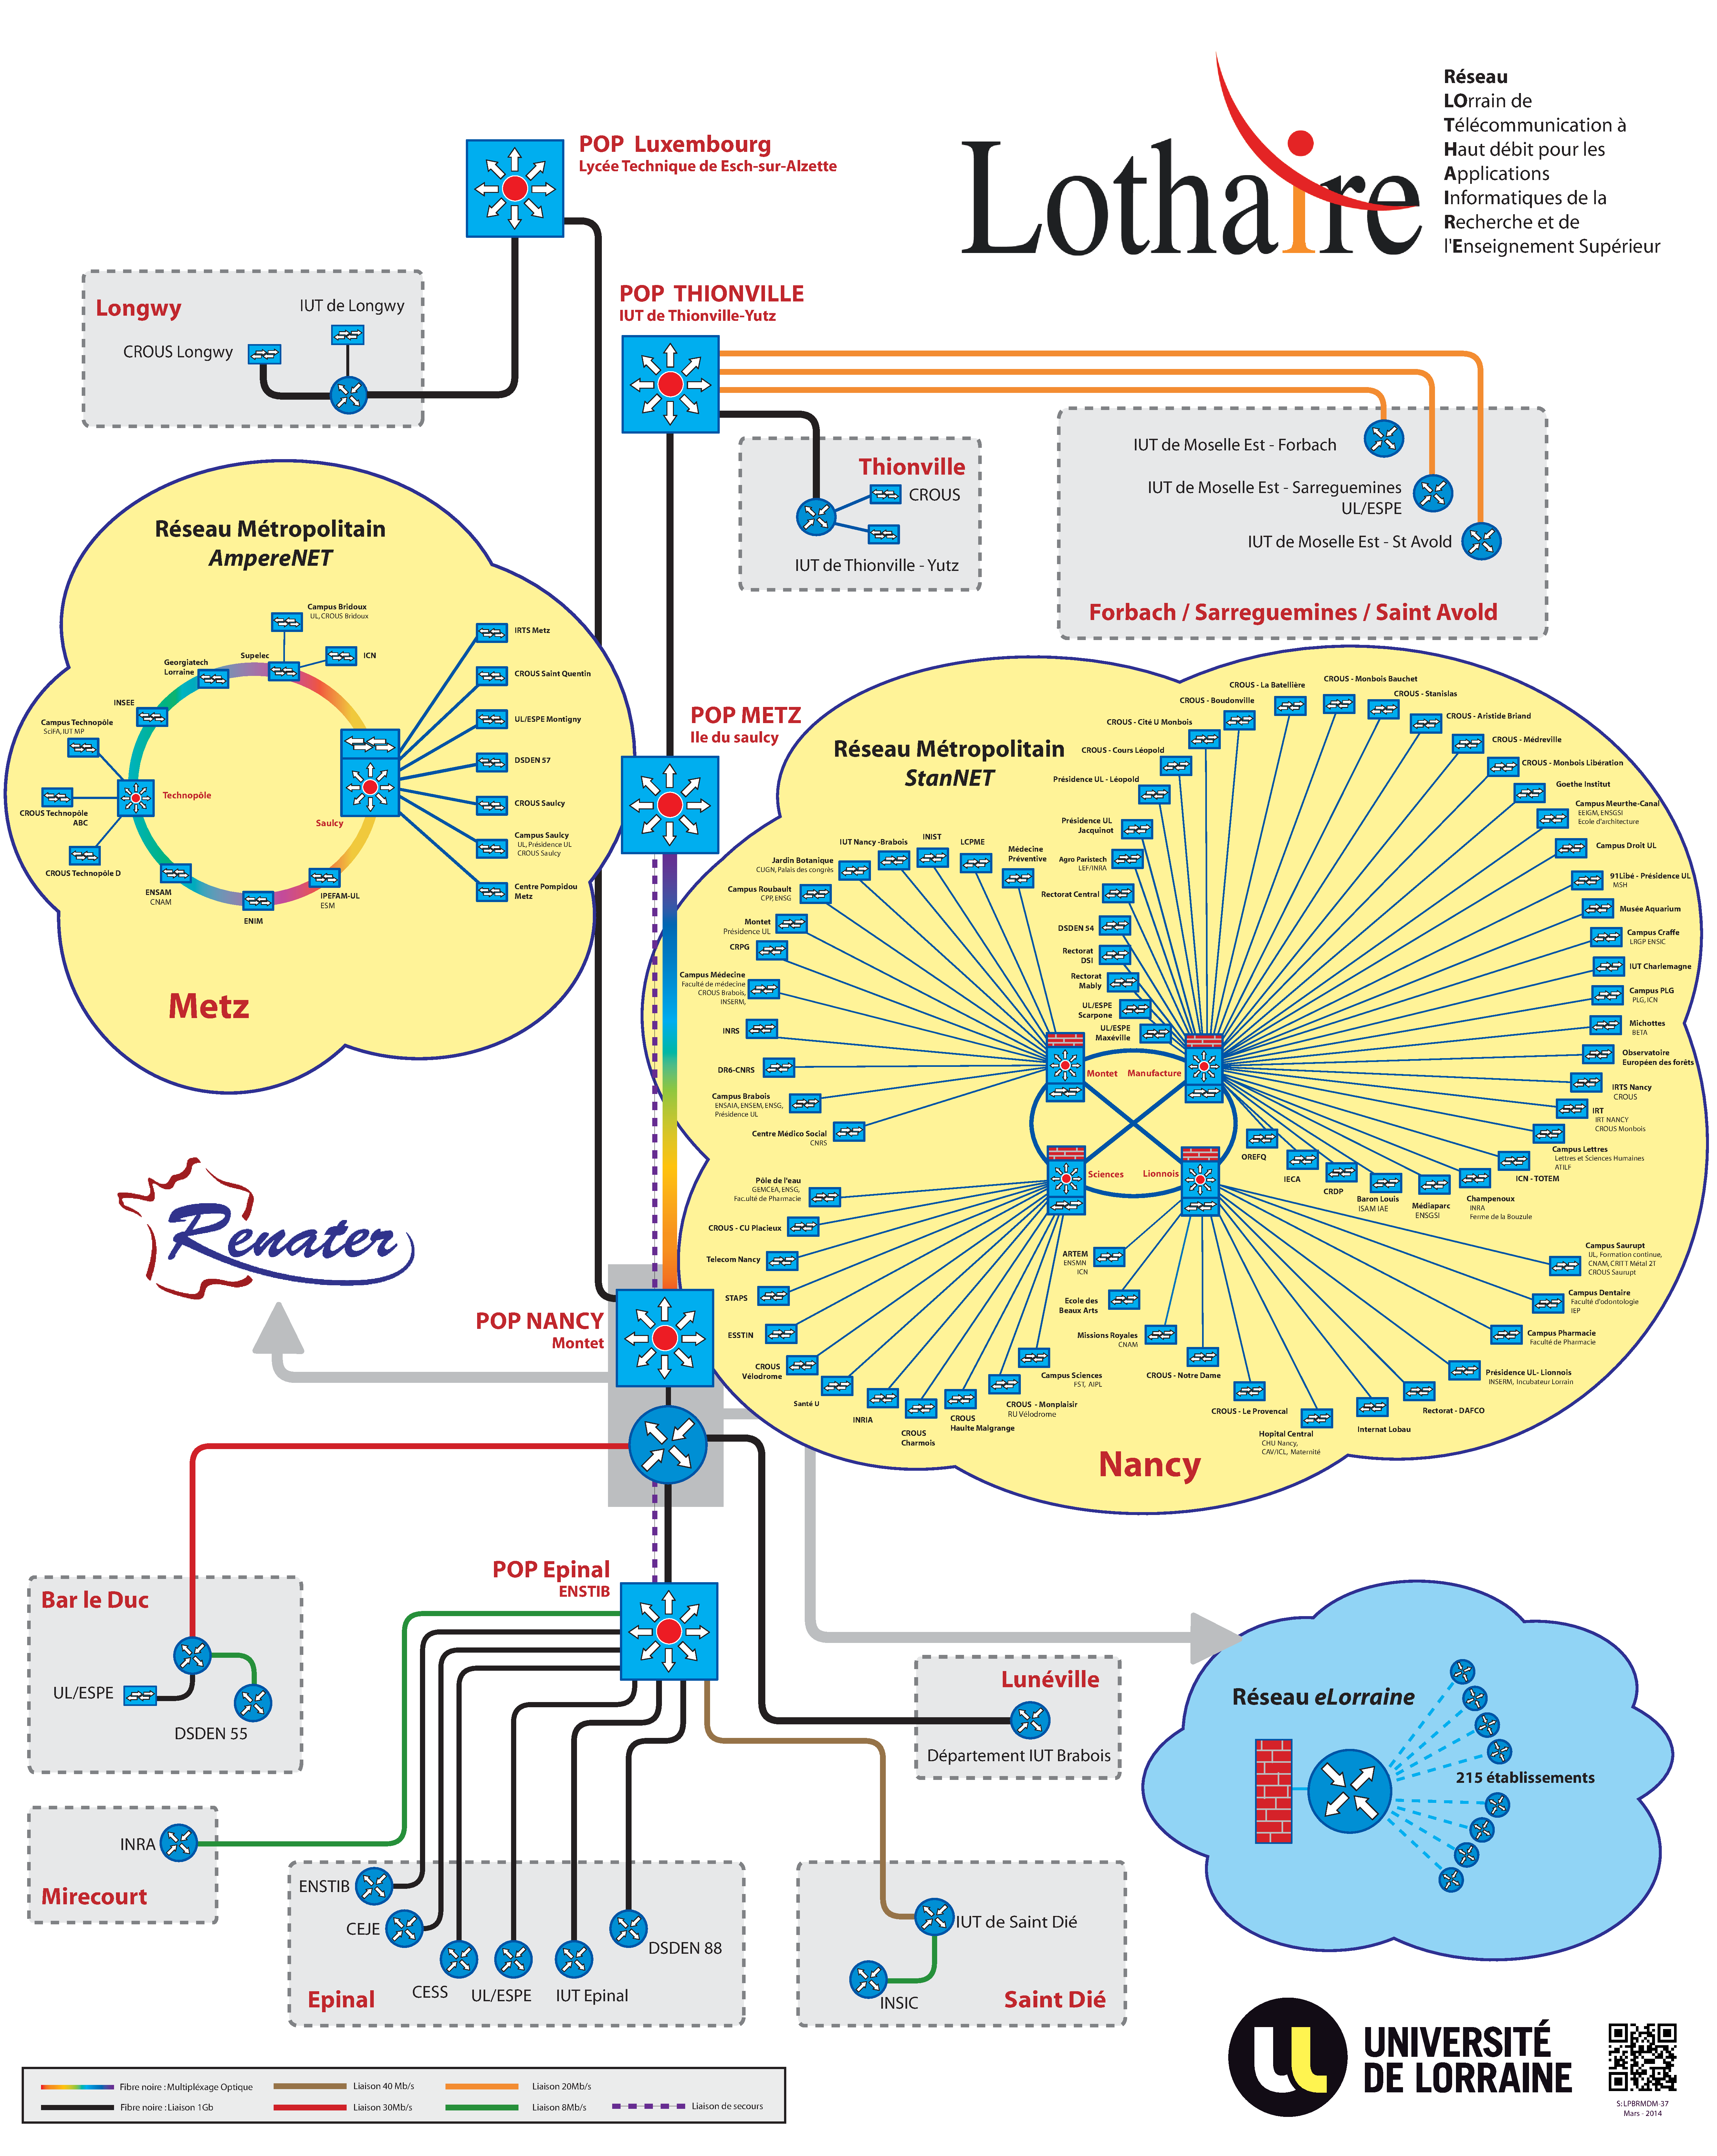
\includegraphics[width=1\textwidth]{poster-lothaire.pdf}
    \label{fig:imagereseaulothaire2}
    \caption{Représentation du réseau Lothaire}
\end{figure}


\section{Images Kibana}
\begin{figure}[H]
\center
\includegraphics[width=0.4\textwidth,height=0.8\textheight]{kibanatuto/rap/4.png}
\label{fig:kibanatuto4}
\caption{Le tableau des champs}
\end{figure}
\paragraph{}
\begin{figure}[H]
\center
\includegraphics[width=0.8\textwidth]{kibanatuto/rap/17.png}
\label{fig:kibanatuto10}
\caption{Choix des visualisations}
\end{figure}
\paragraph{}
\begin{figure}[H]
\center
\includegraphics[width=1\textwidth]{kibanatuto/rap/10.png}
\label{fig:kibanatuto7}
\caption{Visualisations possibles}
\end{figure}
\paragraph{}
\begin{figure}[H]
\center
\includegraphics[width=1\textwidth]{kibanatuto/rap/19.png}
\label{fig:kibanatuto12}
\caption{Dashboard plus avancé}
\end{figure}

\section{Statistiques Munin}
\begin{figure}[H]
\center
\includegraphics[width=1\textwidth]{munin/elk2cpu-month2.png}
\label{fig:elk2cpu}
\caption{Consommation CPU effective mensuel d'Elk2, en bleu\ldots}
\end{figure}
Ne vous esquintez pas les yeux, le bleu est pratiquement indiscernable.

\begin{figure}[H]
\center
\includegraphics[width=1\textwidth]{munin/elk2if_eth0-week.png}
\label{fig:elk2eth0}
\caption{Bande passante Up et Down de Elk2}
\end{figure}
\begin{figure}[H]
\center
\includegraphics[width=0.8\textwidth]{munin/elk1memory-day.png}
\label{fig:elk1memory}
\caption{Utilisation RAM Elk1}
\end{figure}
La ligne orange représente la RAM effectivement utilisée, la zone bleue la mémoire virtuelle.
\begin{figure}[H]
\center
\includegraphics[width=0.8\textwidth]{munin/elk1cpu-day.png}
\label{fig:elk1cpu}
\caption{Utilisation CPU Elk1}
\end{figure}

\chapter{Code Source et scripts}

\lstinputlisting[style=logstash,label={lst:scriptdelindex},caption={Script de suppression d'index}]{../code/remove.sh}

\lstinputlisting[style=logstash,label={lst:scriptkibanaservice},caption={Service simple pour kibana}]{../code/kibana/kibana.service}
Le chemin de l'application est là à titre indicatif, \ipath{/usr/local/bin} est plus 
indiqué, par exemple.


\lstinputlisting[style=logstash,label={lst:scriptfinal},caption={Script de configuration général coté server central}]{../code/logstash/logstashfinal.conf}




\printglossaries

\end{document}
